\documentclass[12 pt]{article}
\usepackage{hyperref, fancyhdr, setspace, enumerate, amsmath,
  lastpage, amssymb, algpseudocode, bussproofs, tikz, listings,
  marvosym, stmaryrd, collectbox}
\usetikzlibrary{shapes.geometric}
\usetikzlibrary{positioning}
\EnableBpAbbreviations
\usepackage[margin=1 in]{geometry}
\allowdisplaybreaks
% \usepackage[dvipsnames]{xcolor}   %May be necessary if you want to color links
\hypersetup{
  % colorlinks=true, %set true if you want colored links
  linktoc=all,     %set to all if you want both sections and subsections linked
  linkcolor=black,  %choose some color if you want links to stand out
}
% New environment to scale prooftrees, from https://tex.stackexchange.com/questions/104554/how-to-scale-prooftree-environment-bussproofs-package
\newenvironment{scprooftree}[1]%
  {\gdef\scalefactor{#1}\begin{center}\proofSkipAmount \leavevmode}%
  {\scalebox{\scalefactor}{\DisplayProof}\proofSkipAmount \end{center}
}
%New command \mybox to box something
\newcommand{\mybox}{%
\collectbox{%
	\setlength{\fboxsep}{3pt}%
	\fbox{\BOXCONTENT}%
	}%
}

\DeclareMathOperator*{\argmax}{arg\!\max}
\DeclareMathOperator*{\argmin}{arg\!\min}

\usepackage{graphicx}
\graphicspath{{Images/}}
\author{Julian Lore}
\date{Last updated: \today}
\title{MATH 423: Regression and Analysis of Variance}
\pagestyle{fancy}
\lhead{MATH 423}
\chead{\leftmark}
\rhead{Julian Lore}
\cfoot{Page \thepage \ of \pageref{LastPage}}
\newcommand{\tab}[1]{\hspace{.2\textwidth}\rlap{#1}}
\newenvironment{rcases}
  {\left.\begin{aligned}}
  {\end{aligned}\right\rbrace}
\begin{document}
\onehalfspacing
\maketitle
\tableofcontents
\section{Introduction}
\begin{itemize}
\item
\textbf{Regression analysis} is about investigating quantitative predictive
relationships variables. Several examples include: getting a car insurance quote. You
provide the company/website a lot of personal information about
yourself and your car and then they'll tell you an estimated price of
your car insurance. How do they get this estimated price? Linear
regression. Another application is estimating your time of arrival
when taking a taxi or some other ride. Credit card applications also
use some form of linear regression to assess the risk of you not
paying your debt, etc. Many asset management pricing models use linear
regression too.
\item
  \textbf{Prediction} is important, which consists of studying the
  relation between two or more variables
\item This class is about:
  \begin{itemize}
  \item Crafting predictive mathematical models
  \item Seeing whether such models really have any predictive power
  \item Comparing their predictions
  \end{itemize}
\end{itemize}
A more concrete example is Sales vs TV, Radio and Newspaper
advertising, with a linear-regression line fit for each. Now we want
to predict sales using all three variables, i.e.\ $Sales \approx
f(TV,Radio,Newspaper)$. Eventually we will study how to estimate this
function $f$ given the data.

Let's go back to a simpler example. Say we only have one variable,
with no other variables, e.g.\ temperature, we want to estimate the
temperature but only have historical data of previous
temperatures. How do we predict tomorrow's temperature? Here we
\textcolor{red}{cannot} use regression, we don't have two
variables. The simplest answer is to use an average. Get the average
of the previous temperatures of the same date of previous years. How
do we generalize this? Given multiple variables but only wanting to
predict one, how do we do so? It will still be some sort of average,
but not simply an average of the output.
\section{Statistical Prediction and\\ Optimal Linear Regression}
\subsection{Predicting a Random Variable from its Distribution}
Let's first think about what the optimal prediction would look like,
if we somehow knew all the probability distribution of our
variable. Suppose we want to predict the value of a random variable
$Y$. What's the best prediction we can make? The best one-number guess
we could make for $Y$ is just its expected value $E(Y)$. Why is this
the case? We want to mathematically show this.

We need some way to measure how good a prediction $m$ is.
\begin{itemize}
\item The difference $Y-m$ should be small
\item Since we don't care about positive more than negative errors, we
  can use $(Y-m)^2$. Since $Y$ is random, this will fluctuate (it is a
  function of a random variable and is thus also a random variable). So we
  use its expected value.
\end{itemize}
  $$MSE(m) = E[(Y-m)^2]$$
  where MSE stands for mean square error. However, sometimes the
  positive and negative error don't have the same importance, like
  predicting bank expenses, you don't want to predict negative
  expenses as you may go bankrupt. In this case the median may be
  better. We will see this case later. Also note that $(Y-m)^2$ is
  called the loss function.

  From the definition of variance:
  \begin{align*}
    MSE(m) & = E[(Y-m)^2] = (E[(Y-m)])^2 + Var[Y-m] = (E[Y]-m)^2 + Var[Y]
  \end{align*}
  We cannot control the variance of $Y$, as it is given to us. We can
  however, do something about $(E[Y] - m)^2$, thus seeing that the
  optimal solution would be $m = E[Y]$.

  But if we don't have all the data on $Y$, then we can estimate
  $E[Y]$ using the sample mean.

Say you have an infinite amount of data, but it is always fluctuating
and you cannot get a hold of a value. How should we estimate it? The
theory tells us to use the expected value. This does not rely on the
actual distribution. However, in reality, we often don't have the full
knowledge of the distribution, we often have discrete measurements,
i.e.\ a histogram. In this case we use the sample mean.

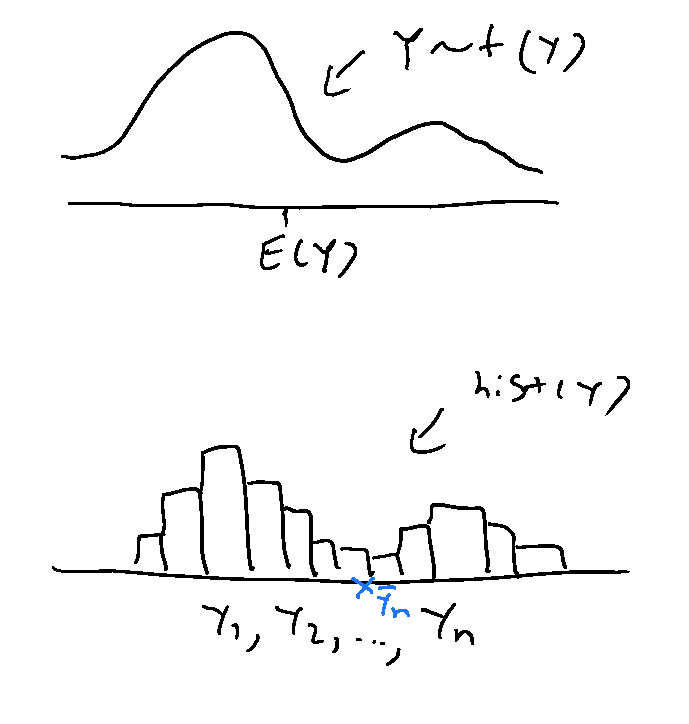
\includegraphics[width=.7\textwidth]{1.pdf}

Looking back at $(E[Y]-m)^2 + Var[Y]$, the first term is the squared
bias of estimating $Y$ with $m$. So we want to choose an $m$ such that
this bias is minimized (should be $0$, as we can set $m=Y$).

The second term is the variance of $Y-m$ (or variance of $Y$, since
$m$ is not random).

This form is called the Bias-Variance decomposition which plays a
central role in machine learning. This isn't only true for just linear
model, it's true for any random variable $Y$.

We would like to pick $m$ to make $MSE(m)$ small. Denote $m^*$ as the
value of $m$ that minimizes $MSE(m)$.
$$m^* = \argmin_m E[(Y-m)^2]$$
$Var(Y)$ is irrelevant to making this small, since it's the same no
matter what $m$ is.

To find the minimum of $MSE(m)$, we denote $\mu = E(Y)$.
\begin{align*}
  \frac{dMSE(m)}{dm} & = \frac{d}{dm} \left[Var[Y] + (\mu - m)^2\right] = \frac{dVar(Y)}{dm} + 2(\mu-m) \left(\frac{d\mu}{dm} - \frac{dm}{dm}\right)
  \\ & = 0 + 2(\mu - m) \left(0 - \frac{dm}{dm}\right) = - 2(\mu - m) = 0
\end{align*}
Therefore
$$m^* = \mu = E(Y)$$
In other words, the best one number guess for $Y$ is just $E(Y)$.

\subsection{Two Variables/Predicting one random variable from another}
Now what about the case in which we have $X$ and $Y$, two random
variables that we can collect data from. Just using the expected value
of $Y$ (say insurance claim) is not fair for the different $x$ (say
age), as everyone will pay the same rate even though different age
groups have different average insurance claims. So we look around a
certain age group using conditional probability, i.e.\ $E[Y|X =
40]$. So we can do this for every value of $X$ and then we get a
\textbf{regression line}.

More formally: we have two random variables, $X$ and $Y$ and their
joint distribution.
\\ We use $X$ to predict $Y$. Our prediction is therefore a function
of $X$, which we'll denote as $m(x)$. What's the best prediction we
can get?
$$m^*(x) = E[Y | X = x]$$
Using the same criterion as the single variable case, we want to
minimize:
$$m^*(\cdot) = \argmin_{m(\cdot)} E_{X,Y}[(Y-m(x))^2]$$
If we denote $\mu(x) = E_{Y|X}[Y|X = x]$ to represent the conditional
expectation of $Y$ given $X = x$. We will prove that
$$m^*(x) = \mu(x)$$
\paragraph{Proof:}
\begin{align*}
  E_{X,Y}[(Y-m(x))^2] & = E_{X}[E_{Y|X}[(Y-m(x))^2 | X]]
\end{align*}

We can call the left hand side the loss function, or the
generalization error.

For the inner expectation, for each possible value of $X = x$, the
optimal value $m^*(x)$ is just the conditional mean (since $x$ is a
constant when conditioned on):
$$m^*(x) = \mu(x) = \underbrace{E_{Y|X}[Y|X = x]}_{\text{regression function}}$$

In terms of estimation, if you want to get the optimal value at $X=4$,
you need lots of observations at $X=4$ to approximate the expected
value of $Y$ given $X = 4$. If we don't have lots of observations, we
use the point's $k$-nearest neighborhood, include extra points around $X =
4$ to estimate the expectation. This performs pretty well in
general. However in the higher dimension cases, a small neighborhood
will include less points, so you have less points to average and might
not be able to use this method.

There are many possible forms for $E[Y \mid X = x]$, such as:
\begin{align*}
  E[Y \mid X = x] & = x^T \beta & \text{linear regression}
  \\ E[Y \mid X = x] & = T_0(x) & \text{Regression tree}
  \\ E[Y \mid X = x] & = \sum_{t=1}^{T}T_{0,t}(x) & \text{Random Forest}
  \\ E[Y \mid X = x] & = \sum_{i=1}^n \alpha_{ik}(x_i, k) &
                                                            \text{support
                                                            vector machine}
\end{align*}
\paragraph{$k$-nearest neighborhood (KNN)} (side topic, not directly related
to linear regression, but very important, linear regression is the
strictest model, whereas the nearest neighborhood model is the least
strict, you don't rely on a distribution or anything, whereas the
linear regression model relies heavily on a distribution)

Goal: to estimate the conditional distribution of $Y$ given $X$. $X
\in \mathbb{R}^p$, $p \geq 1$ (i.e.\ $X$ can be higher dimensional, a
vector). Specifically, $E[Y | X = x]$. Given a positive integer $K$
and a test observation $x_0$, the procedure is as follows.
\\ Procedure: KNN
\begin{itemize}
\item First identify $K$ points in the training data that are closest
  to $x_0$, represented by $N_0$.
\item Then estimate $$\hat{E}[Y | X = x_0] = \frac{1}{k} \sum_{i \in N_0}y_i$$
  (the hat signifies an estimation)
\end{itemize}
\paragraph{Example}
\begin{tabular}{l l l l l}
  \hline Observation& $X_1$& $X_2$&$X_3$&$Y$
  \\ \hline $x_1$ & $0$ & $3$ & $0$ & $1$
  \\ $x_2$ & $2$ & $0$ & $0$ & $2$
  \\ $x_3$ & $0$ & $1$ & $3$ & $3$
  \\ $x_4$ & $0$ & $1$ & $2$ & $4$
  \\ $x_5$ & $-1$ & $0$ & $1$ & $5$
  \\ $x_6$ & $1$ & $1$ & $1$ & $6$
\end{tabular} This is our \textbf{training data}.
\\ Suppose we want to use this data set to make a prediction for $Y$
when $x = (x_{01}, x_{02}, x_{03}) = (0, 0,0)$ using $K$-NN.\
\begin{enumerate}[(a)]
\item Compute the Euclidean distance between each observation and the
  test point, $x_0$.
  \begin{itemize}
  \item $\left\lVert x_1 - x_0 \right\rVert_2 = \sqrt{(0-0)^2 +
      (3-0)^2 + (0-0)^2} = 3$
  \item $\left\lVert x_2 - x_0 \right\rVert_2 = 2$
  \item $\left\lVert x_3 - x_0 \right\rVert_2 = \sqrt{10}$
  \item $\left\lVert x_4 - x_0 \right\rVert_2 = \sqrt{5}$
  \item $\left\lVert x_5 - x_0 \right\rVert_2 = \sqrt{2}$
  \item $\left\lVert x_6 - x_0 \right\rVert_2 = \sqrt{3}$
  \end{itemize}
\item Now we can get a prediction for any hyper parameter $k$. What is
  the prediction with $k = 1$? $x_5$ is closest to $x_0$ so our
  prediction is $Y = 5$.
\item $k = 3$, $\frac{1}{3} (2 + 5 + 6) = \frac{13}{3}= 4 \frac{1}{3}$
\end{enumerate}
So this method is very flexible as it does not rely on any
distribution. However, it becomes very difficult to find the optimal
$k$ and the performance of the algorithm gets worse as we increase the
dimension. Though in many cases, this is still the best method to
use. Often people use a combination of this method and linear models.

\subsection{The Optimal Linear Predictor}
Unfortunately, in general $m(x)$ is a really complicated function for
which there exists no nice mathematical expression. We could
substitute a simplified model for the relationship for
the actual relation.

We restrict the prediction function $m(x)$ to have the linear form,
i.e.\ $$m(x) = \beta_0 + \beta_1 x$$
Now we want to know what the optimal prediction we can make which is
linear in $X$?

To minimize the mean squared error of $m(x) = \beta_0 + \beta_1 x$
\begin{align*}
  (\beta_0^*, \beta_1^*) & = \argmin_{(\beta_0, \beta_1)} E_{X, Y}[(Y - \underbrace{(\beta_0 + \beta_1 x)}_{m(x)})^2]
  \\ E[(Y - (\beta_0 + \beta_1 x))^2] & = E[Y^2] - 2 \beta_0 E[Y] - 2 \beta_1 E[XY] + E [ (\beta_0 + \beta_1 x)^2]
  \\ & = E [Y^2] - 2\beta_0 E[Y] -  2\beta_1 (Cov (X,Y) + E[X]E[Y]) + \beta_0^2 + 2\beta_0\beta_1 E[X] + \beta_1^2 E[X^2]
  \\ & = E[Y^2] - 2 \beta_0 E[Y] - 2 \beta_1 (Cov(X,Y) + E[X]E[Y]) + \beta_0^2 + 2 \beta_0 \beta_1 E[X]
  \\ & + \beta_1^2 (Var(X) + E[X]^2)
\end{align*}
Now to get the optimal values, we take the derivative:
\begin{align*}
  \frac{\partial{E[Y - (\beta_0+\beta_1X)^2]}}{\partial{\beta_0}} & = -2E[Y] + 2 \beta_0 + 2\beta_1 E[X] = 0
\end{align*}
This gives us:
$$\beta_0^* = E[Y] - \beta_1^* E[X] \iff E[Y] = \beta_0^* + \beta_1^*
E[X]$$
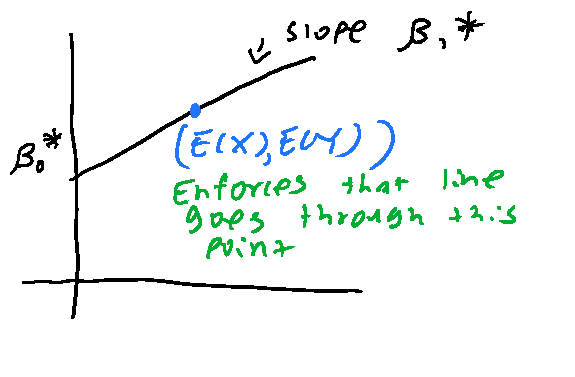
\includegraphics[width=.9\textwidth]{2.pdf}
\begin{itemize}
\item The optimal intercept $\beta_0^*$ ensures that the line goes
  through $E[Y]$ at the $E[X]$ value.
\item If the variables were centered with $E[Y] = E[X] = 0$ then
  $\beta_0^* = 0$.
\end{itemize}
\begin{align*}
  \frac{\partial{E[Y]-(\beta_0+\beta_1X)^2}}{\partial{\beta_1}} & = -2Cov(X,Y) - 2E[X]E[Y] + 2\beta_0E[X] + 2\beta_1 Var(X) + 2\beta_1 (E[X])^2
                                                                  \intertext{Plug
                                                                  in
                                                                  $\beta_0^*
                                                                  =
                                                                  E[Y]
                                                                  -
                                                                  \beta_1^*
                                                                  E[X]$}
  & = -Cov(X,Y) + \beta_1 Var(X) = 0
  \\ \beta_1^* & = \dfrac{Cov(X,Y)}{Var(X)}
\end{align*}
\begin{itemize}
\item Since the optimal slope $\beta_1^*$ is $\frac{Cov(X,Y)}{Var(X)}$
  (ratio), the slope increases the more $X$ and $Y$ tend to fluctuate
  together, and gets smaller/closer to zero the more $X$ fluctuates.
  \\ 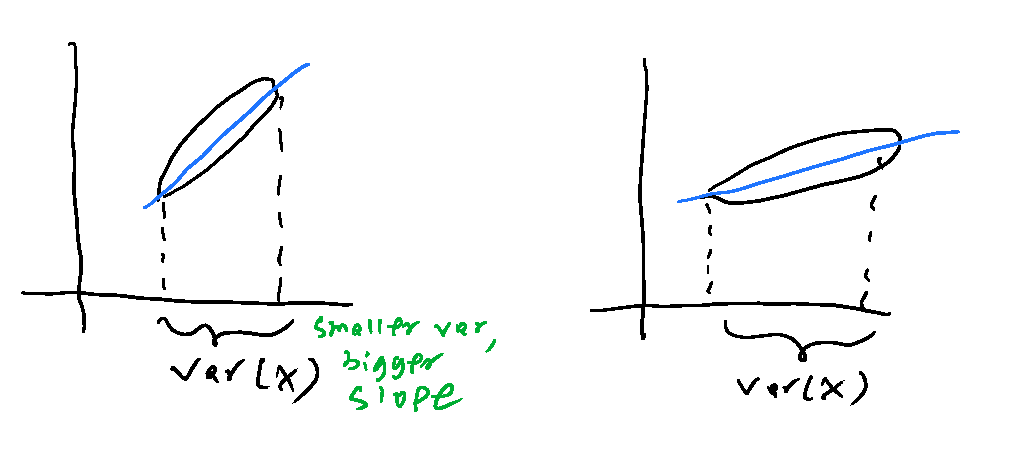
\includegraphics[width=.9\textwidth]{3.pdf}
\item $\beta_1^*$ doesn't change if we use $X' = X-a, Y' = Y - b$
  instead. Note that $a$ and $b$ must be deterministic/non-random.
\end{itemize}
Eventually you will get the \textbf{optimal regression line} (of $Y$
on $X$):
$$m^*(x) = \beta_0^* + \beta_1^* x$$
\begin{itemize}
\item At no time did we have to assume that the actual relationship
  between $X$ and $Y$ is linear (that's just our belief, it may not
  actually be linear). We only have an optimal linear approximation to
  the \textbf{true relationship}, whatever it might be. Your data
  might even look like:
  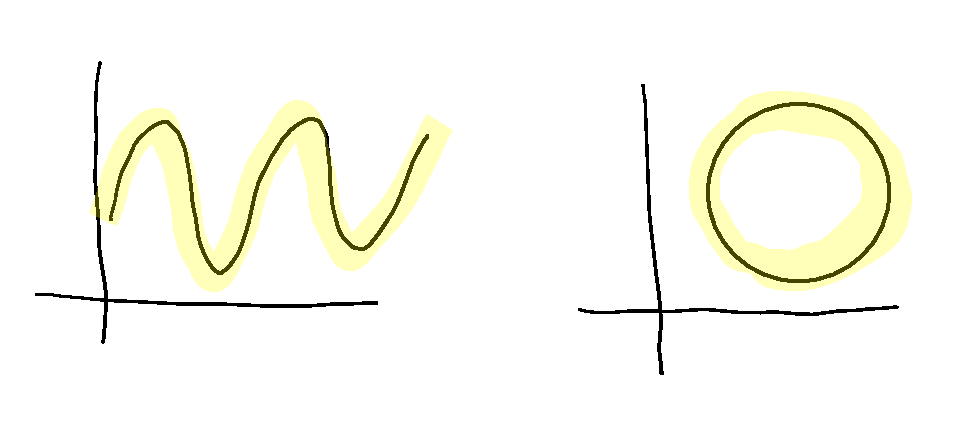
\includegraphics[width=.9\textwidth]{4.pdf}
  % \\ However, in this case linear regression will fail and a more
  % general method is required.
\item The best linear approximation to the truth can be awful. Imagine
  $$E[Y | X = x] = e^x \text{ or } \sin(X)$$
  There is no general reason to think linear approximation ought to be
  good. But \underline{sometimes} it works. For example, the true
  regression function of the above would be $E[Y | X = x] = e^x$,
  which is differentiable and can be approximated using a polynomial
  of $X$ (Taylor expansion).
  \begin{align*}
    e^x & = e^{x_0}+ \frac{de^X}{dx} \vline_{x = x_0}(x - x_0) + \frac{1}{2} \frac{d^2e^x}{dx^2}\vline_{x = x_0} (x-x_0)^2 + \ldots
    \\ & = e^{x_0} + e^{x_0}(x-x_0) + \frac{1}{2}e^{x_0}(x-x_0)^2 + \ldots
  \end{align*}
\item If $x$ is close enough to $x_0$ then $$e^x \approx e^{x_0} +
  e^{x_0}(x-x_0) = e^{x_0} (1- x_0) + e^{x_0}x$$
  In this case our linear approximation would just be the first two
  terms.

  How close is close enough? The first two terms should dominate the
  remaining terms (quadratic cubic), i.e.
  $$e^{x_0} |x - x_0| >> \frac{1}{2} e^{x_0} |x - x_0|^2 \iff 2
  \frac{e^{x_0}}{e^{x_0}} >> \frac{|x-x_0|^2}{|x-x_0|} \iff 2 >> |x -
  x_0|$$
  So $x \in (x_0 - 2, x_0 + 2)$ at least.
\end{itemize}
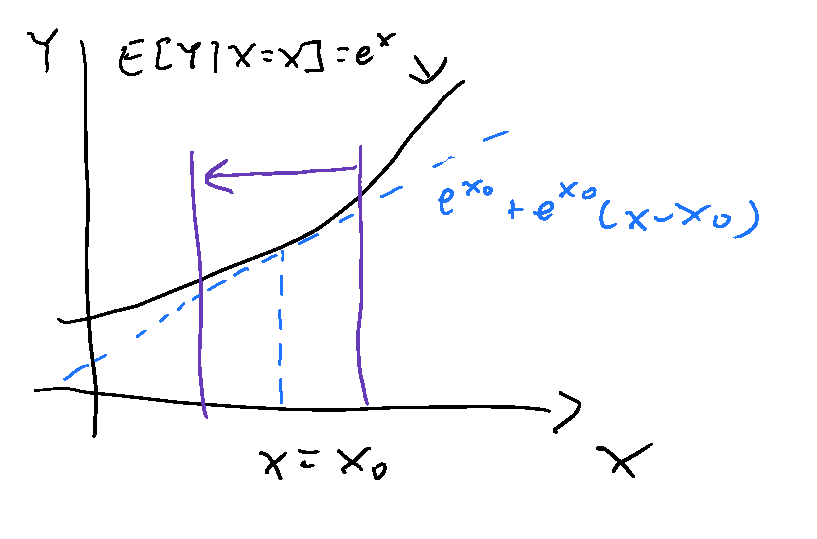
\includegraphics[width=.9\textwidth]{5.pdf}
\begin{itemize}
\item
Linear regression isn't always the best method of approximation,
however it is easy to do and is one of the main methods that is
computationally efficient for high dimension problems or if you want
to approximate many points, sometimes more than the number of
observations you have.
\item We don't assume that $X$ came before $Y$ in time, that $X$
  causes $Y$ or that $X$ is known precisely but $Y$ only noisily to
  get the optimal linear prediction.
\item At no time did we have to specify the marginal distribution of
  $X$ and $Y$, or about the joint distribution of $X$ and $Y$.
\item At no time did we have to assume anything about the fluctuation
  of $Y$ being Gaussian or symmetric.
\end{itemize}
\section{Simple Linear Regression Model}
\subsection{Notation}
We consider two types of variables.
\begin{itemize}
\item ``Output'': $Y$ \hbox{--} measured outcome of interest. Can also be
  called outcome or response variable.
\item ``Input'': $X$ \hbox{--} variable(s) that correlated to the variation in
  the ``Output''. Can also be called features, covariates/factors or
  predictors.
\end{itemize}
Both variables will be measured during the study.
\subsection{Model Setup}
The simple linear regression has two variables $X$ and $Y$ where we
try to predict $Y$ from $X$. The assumptions of the model are as
follows (this definition is more general than the one in the textbook,
however we will see a more developed one more comparable to the
textbook later):
\begin{enumerate}
\item The distribution of $Y$ is arbitrary (and perhaps $X$ is
  non-random)
\item If $X = x$ (it is given/we observe a value of $x$), then $Y =
  \beta_0 + \beta_1 x + \varepsilon$ for some constants $\beta_0$ and
  $\beta_1$ and some random noise.
  \\ Why not just use $Y = \beta_0 + \beta_1 x$? Often the
  relationship between two variables is not deterministic, for
  example, the effects of smoking can vary from person to person,
  although they may have the same value for $x$ (like age).
\item $E[\varepsilon \mid X = x] = 0 = E[\varepsilon]$ and
  $Var(\varepsilon \mid X = x) = Var(\varepsilon) =
  \sigma^2 > 0$ (constant).
\item $\varepsilon$ is uncorrelated with $X$ (i.e.\ $Cov(\varepsilon,
  X) = 0$) and is \textbf{uncorrelated across observations}.

  (This will most likely be a final exam question)
\end{enumerate}
Visually, this model:\\
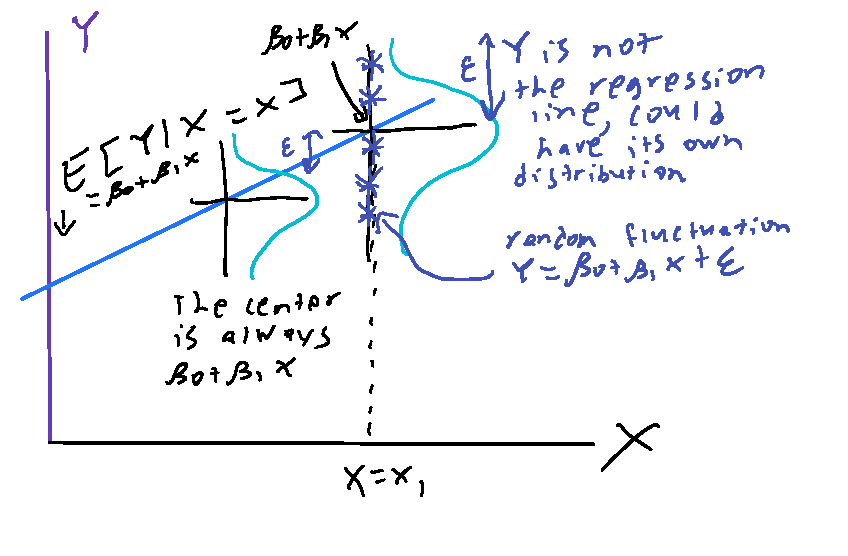
\includegraphics[width=.9\textwidth]{6.pdf}
\begin{align*}
  E[\varepsilon \mid X = x] & = E[\varepsilon] = 0
  \\ Var[\varepsilon \mid X = x] & = Var[\varepsilon] = \sigma^2
\end{align*}
$\varepsilon$ is independent to $X$.
\\ Essentially, we have a distribution (any distribution satisfying
the expectation and variance above) centered at every point
of the regression line.
\\ In 3D:
\\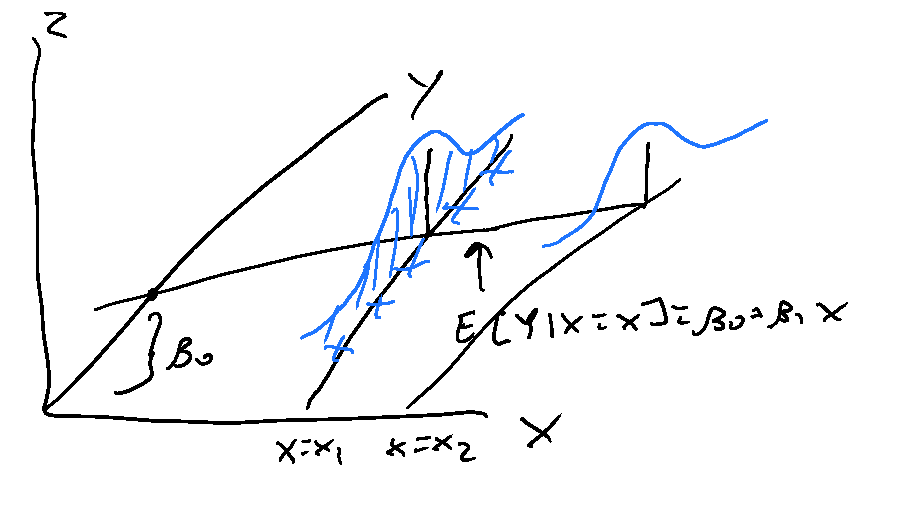
\includegraphics[width=.5\textwidth]{7.pdf}
\\
\\ The points are more dense near the center of the distribution. If
the distribution is bimodal, the data will be dense at the two peaks.
\\ 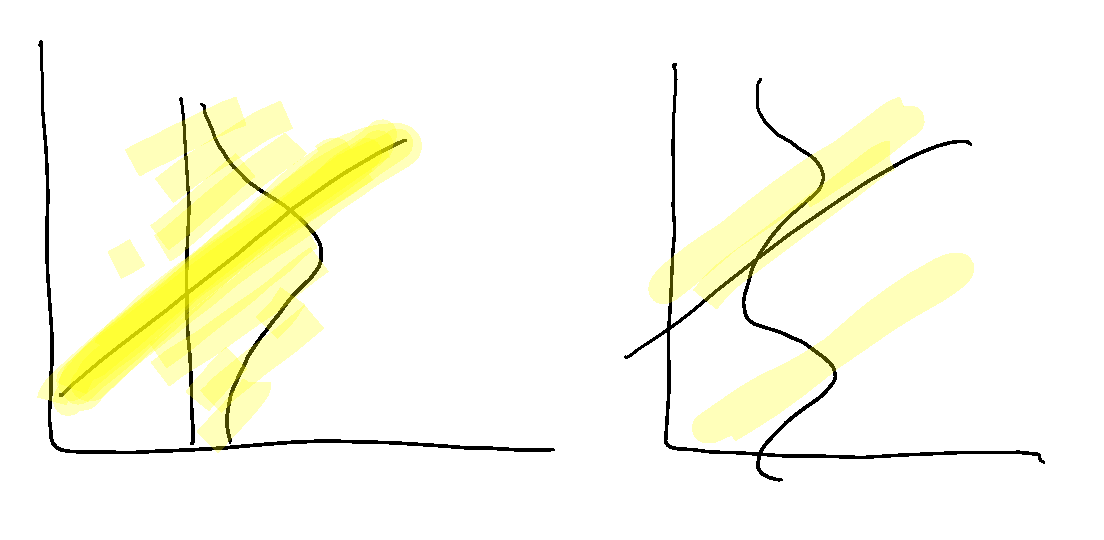
\includegraphics[width=.9\textwidth]{8.pdf}
\\
Note that:
\begin{enumerate}
\item The assumption is equivalent to assuming that the
  \textbf{regression function is linear}.
  \begin{align*}
  E[Y \mid X = x] & = E [\beta_0 + \beta_1 X + \varepsilon | X = x] =
                    \beta_0 + \beta_1x
    \\ Var[Y \mid X = x] & = Var[\underbrace{\beta_0+\beta_1X}_{\text{constant} \implies Var = 0} + \varepsilon \mid X = x ] = Var[\varepsilon \mid X = x] = \sigma^2
  \end{align*}
\item The noise variable $\varepsilon$ may represent
  \textbf{measurement error or fluctuation} in $Y$ or some combination
  of both.
\item The assumption of additive noise ($\varepsilon$ is just added to
  the function) is non-trivial \hbox{--} it's
  not absurd to imagine that it could be multiplicative.
\item \textbf{Linear functional form}, constant variance is not
  trivial.
\item But the assumption that noise has mean $0$ is trivial.
  \begin{align*}
    E [\varepsilon \mid X = x] & = c,\ \varepsilon' = \varepsilon - c,\ E[\varepsilon' \mid X = x] = 0
    \\ \implies Y & = (\beta_0 + c) + \beta_1 x + \varepsilon'
  \end{align*}
\end{enumerate}
With multiple data points $(X_1, Y_1), (X_2,Y_2), \ldots, (X_n,Y_n)$
(capitalized, these could be different random variables/different
distributions, they are random until we actually sample them)
then the model says that for each $i = 1, \ldots, n$
$$Y_i = \beta_0 +\beta_1 X_i + \varepsilon_i$$
where the noise variable $\varepsilon_i$ all have the same expectation
($0$) and same variance ($\sigma^2$) and $Cov(\varepsilon_i,
\varepsilon_j) = 0$ for $i \neq j$ (uncorrelated across observations
as mentioned earlier). $Cov(\varepsilon_i, \varepsilon_i) =
Var(\varepsilon_i) = \sigma^2$
\\ Equivalently, the assumption says that $E[Y_i \mid X_i = x_i] =
\beta_0 +\beta_1 x_i$ for $i = 1, \ldots, n$ and constant variance
across $i$ $$Var(Y_i \mid X_i = x_i) = \sigma^2$$ for $i = 1, \ldots,
n$ and $Y_i$'s are \textbf{conditionally independent given $X_i$'s} because
\begin{align*}
  Cov(Y_i, Y_j \mid X_i = x_i, X_j = x_j) &
                                            \stackrel{\beta_0+\beta_1X_i
                                            \text{ constant given }x_i}{=} Cov(\varepsilon_i, \varepsilon_j \mid X_i = x_i, X_j = x_j)
  \\ & = Cov(\varepsilon_i, \varepsilon_j) = 0
\end{align*}
But we find that $Y_i$'s are \textbf{not unconditionally independent}.
\begin{align*}
  Cov(Y_i, Y_j) & = Cov(\beta_0 + \beta_1 X_i + \varepsilon_i, \beta_0 + \beta_1X_j + \varepsilon_j)
  \\ & = \beta_1^2 Cov(X_i,X_j)+\beta_1 Cov(X_i, \varepsilon_j) + \beta_1 Cov(X_j, \varepsilon_i) + Cov(\varepsilon_i, \varepsilon_j)
  \\ & = \beta_1^2 Cov(X_i, X_j) + 0 + 0 + 0 = \beta_1^2Cov(X_i,X_j)
\end{align*}
\subsection{Plugin estimates}
Remember we saw last time that the optimal linear predictor of $Y$
from $X$ has slope
\begin{align*}
  \beta_1^* & = \dfrac{Cov(X,Y)}{Var(X)}
              \intertext{and intercept}
              \beta_0^* & = E[Y] - \beta_1^* E[X]
\end{align*}
But both $Cov(X,Y)$ and $Var(X)$ are functions of the true
distribution of $(X,Y)$. Rather than having that full distribution, we
merely have data points or \textbf{samples} $(x_{11},y_1),
(x_{21},y_{2}), \ldots, (x_{n1},y_n)$. The additional subscript is to
indicate which $x$ we are talking about, although currently we are
doing simple linear regression with only one predictor, but in the
future we will have multiple.

How might we estimate $\beta_0^*$ and $\beta_1^*$ from this data? (We
will see three methods, here's the first)

Use ``plug-in principle'', plug-in \textbf{sample covariance} and
\textbf{sample variance}. Define:
\begin{align*}
  S_{xx} & = \sum_{i=1}^n (x_{i1} - \overline{x}_1)^2 & \overline{x}_1 = \frac{1}{n}\sum_{i=1}^n x_{i1}
  \\ & = \sum_{i=1}^n(x_{i1} - \overline{x}_1)x_{i1}
  \\ & = \sum_{i=1}^n x_{i1}^2 - n(\overline{x}_1)^2
  \\ S_{yy} & = \sum_{i=1}^n (y_i - \overline{y})^2
  \\ & = \sum_{i=1}^n (y_i - \overline{y}) (y_i - \overline{y}) & \overline{y} = \frac{1}{n}\sum_{i=1}^ny_i
  \\ & \ldots = \sum_{i=1}^n (y_i - \overline{y})y_i
  \\ & = \sum_{i=1}^n y_i^2 - n(\overline{y})^2
  \\ S_{xy} & = \sum_{i=1}^n (y_i - \overline{y})(x_{i1}-\overline{x}_1)
  \\ & = \sum_{i=1}^n(x_{i1} - \overline{x}_1)y_i
  \\ & = \left(\sum_{i=1}^nx_{i1}y_i\right) - n \overline{x}_1 \overline{y}
\end{align*}
You can show these results and their intermediate steps using
\begin{align*}
  \sum_{i=1}^n (x_{i1} - \overline{x}_1) & = 0
  \\ \sum_{i=1}^n (y_i - \overline{y}) & = 0
\end{align*}
(will have to do on assignment).

The plug-in estimate for $\beta_1$ is
\begin{align*}
  \hat{\beta}_1 & = \dfrac{\widehat{Cov}(X,Y)}{\widehat{Var}(X)} \textcolor{blue}{\approx \dfrac{Cov(X,Y)}{Var(X)} = \beta_1^*}
  \\ &                  = \dfrac{\frac{1}{n} \sum_{i=1}^n (y_i - \overline{y})(x_{i1}-\overline{x}_1)}{\frac{1}{n}\sum_{i=1}^n(x_{i1}-\overline{x}_1)^2} = \frac{S_{xy}}{S_{xx}}
  \\ \hat{\beta}_0 & = \hat{E}[Y] - \hat{\beta}_1 E[X] \textcolor{blue}{\approx E[Y] - \beta_1^* E[X]}
  \\ & = \overline{y} - \hat{\beta}_1 \overline{x}_1 = \overline{y} - \frac{S_{xy}}{S_{xx}}\overline{x}_1
\end{align*}
In a more advanced statistics course, you will see that $n \to \infty
\implies \hat{\beta}_1 \to \beta_1^*$ and $\hat{\beta}_0 \to
\beta_0^*$
\subsection{Least square estimates}
There is an alternative way of estimating the simple linear regression
model. Recall that the true optimal slope and intercept are the ones
which minimize the mean squared error
\begin{align*}
  (\beta_0^*, \beta_1^*) & = \argmin_{(\beta_0,\beta_1)} \underbrace{E_{XY} [(Y - \beta_0 - \beta_1 X)^2]}_{\text{unknown}}
\end{align*}
This is a function defined on the distribution of $(X,Y)$, so we can't
get it from the data, but we can approximate it with the data. The
\textbf{in-sample, empirical} or \textbf{training MSE}
\begin{align*}
  S(\beta_0, \beta_1) & = \widehat{MSE}(\beta_0, \beta_1) =
                        \underbrace{\frac{1}{n} \sum_{i = 1}^n (y_i -
                        \beta_0 - \beta_1 x_{i1})^2}_{\text{computable
                        from data}}
\end{align*}
Essentially, we replace the expectation with the sample mean.

If our sample points $(x_{11}, y_1), (x_{21}, y_2), \ldots,
(x_{n1},y_n)$ are all independent for any fixed $(\beta_0, \beta_1)$,
then we find $\hat{\beta}_0, \hat{\beta}_1$ instead of $\beta_0^*$
and $\beta_1^*$.
\begin{align*}
  (\hat{\beta}_0, \hat{\beta}_1) & = \argmin_{\beta_0, \beta_1} \frac{1}{n} \sum_{i=1}^n (y_i - \beta_0 - \beta_1 x_{1i})^2
\end{align*}
These are different from the optimal $\beta_0^*, \beta_1^*$, as we
only observe some points and make a line from them, not the line
centered about all points. Theoretically, they'd only be the same if
we had infinite points, so in general they are never the same. Due to
random fluctuation, rerunning an experiment can give you different
data and thus a different regression line.

The law of large numbers tells us that if $n \to \infty$, then
\begin{align*}
  \widehat{MSE}(\beta_0, \beta_1) & \to MSE(\beta_0, \beta_1)
  \\ \implies (\hat{\beta}_0, \hat{\beta}_1) & \stackrel{n \to \infty}{\to} (\beta_0^*, \beta_1^*)
\end{align*}
To solve $(\hat{\beta}_0, \hat{\beta}_1)$:
\begin{align*}
  \frac{\partial{s}}{\partial{\beta_0}} & = \frac{1}{n}(-2) \sum_{i=1}^n (y_i - \hat{\beta}_0 - \hat{\beta}_1x_{1i}) = 0
  \\ \frac{\partial{s}}{\partial{\beta_1}} & = \frac{1}{n}(-2) \sum_{i=1}^n (y_i - \hat{\beta}_0 - \hat{\beta}_1x_{1i})x_{1i} = 0
\end{align*}
We call these equations \textbf{the normal equations} and can be
rewritten as:
\begin{align*}
  \overline{y} - \hat{\beta}_0 - \hat{\beta}_1 \overline{x}_1 & = 0
  \\ \sum_{i=1}^nx_{1i}y_{i} - \hat{\beta}_0 \overline{x}_1 - \hat{\beta}_1 \sum_{i=1}^n x_{i1}^2 & = 0
\end{align*}
The first equation gives us $$\hat{\beta}_0 = \overline{y} -
\hat{\beta}_1 \overline{x}_1$$ Substituting this into the second equation, we get:
\begin{align*}
  & \frac{1}{n}\sum_{i=1}^nx_{1i}y_i - \overline{y}\overline{x}_1 + \hat{\beta}_1 \overline{x}_1 \overline{x}_1 - \frac{1}{n}\hat{\beta}_1 \sum_{i=1}^n x_{1i}^2 = 0
  \\ &S_{xy} - \hat{\beta}_1 S_{xx} = 0
  \\ &\hat{\beta}_1 = \frac{S_{xy}}{S_{xx}}
\end{align*}
This shows that the least-squares estimates are the same as the plugin
estimates.
\\ 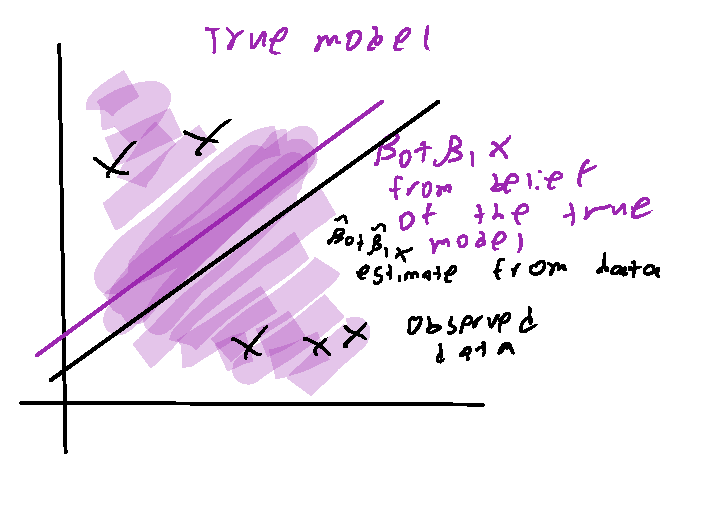
\includegraphics[width=.9\textwidth]{9.pdf}
\\ See \href{http://www.math.mcgill.ca/yyang/regression/comp/Comp-02-SLR_simulation.pdf}{\texttt{Comp-02-SLR\_simulation.pdf}} on the course webpage for more
information, with some example sampling and corresponding regression
lines.
\\
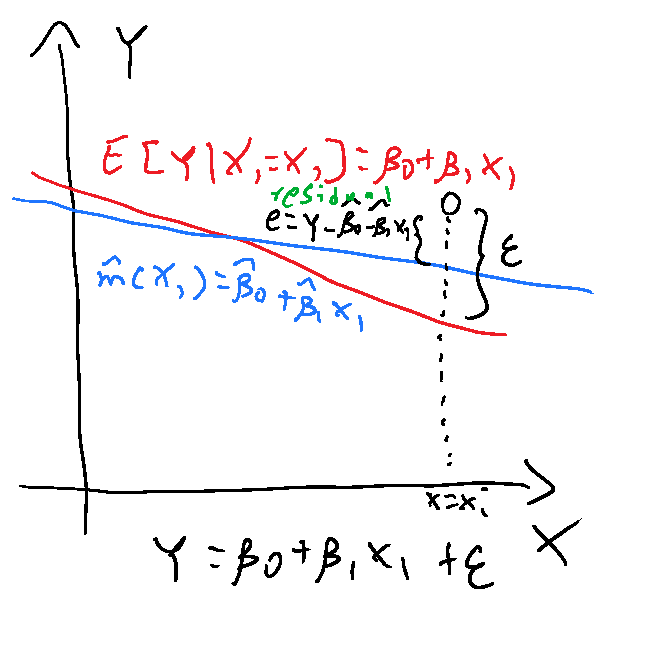
\includegraphics[width=.6\textwidth]{10.pdf}
\\ The red line will go through the population mean, $(E[X], E[Y])$,
whereas the blue line will go through the sample mean, $(\overline{x}_1,
\overline{y})$.
\\If random variables $(X_1, Y)$ are from
$$Y = \underbrace{\beta_0}_{1} + \underbrace{\beta_1}_5 x_1 +
\varepsilon$$
What is the value of $\beta_0^*, \beta_1^*$ such that
\begin{align*}
(\beta_0^*, \beta_1^*) & = \argmin_{\beta_0, \beta_1} E_{X,Y} [(Y -
\beta_0 - \beta_1 X_1)^2]
 \\ \beta_1^* & = \frac{Cov(Y,X_1)}{Var(X_1)}
  \\ \beta_0^* & = E[Y] - \beta_1^* E[X]
\end{align*}
Now plug-in $Y = \beta_0 + \beta_1 X_1 + \varepsilon$:
\begin{align*}
  \beta_1^* & = \frac{Cov(Y, X_1)}{Var(X_1)} = \frac{Cov(\beta_0 + \beta_1 X_1 + \varepsilon, X_1)}{Var(X_1)}
  \\ & = \frac{\beta_1 Var(X_1)}{Var(X_1)} = \beta_1 = 5
  \\ \beta_0^* & = E[Y] - \beta_1^* E[X_1] = E[\beta_0 + \beta_1X_1 + \varepsilon] - \beta_1 E[X_1]
  \\ & = \beta_0 + \beta_1 E[X_1] + 0 - \beta_1 E[X_1]
  \\ & = \beta_0 = 1
\end{align*}
\subsection{Least Squares in Matrix Format}
We have the simple linear regression model
\begin{align*}
  Y & = \beta_0 + \beta_1 X + \varepsilon
\end{align*}
where $E[\varepsilon \mid X = x] = 0$ and $Var(\varepsilon \mid X = x)
= \sigma^2$ and $\varepsilon$ is uncorrelated with $X$ and
uncorrelated across observations.

Say our data consists of $n$ paired observations of $X$ and $Y$,
sampled from the above model
$$(X_1, Y_1), \ldots, (X_n, Y_N)$$
hence
\begin{align*}
  Y_i &= \beta_0 + \beta_1 X_i + \varepsilon_i, i = 1, \ldots, n
\end{align*}
If we denote
\begin{align*}
  Y & =
      \begin{bmatrix}
        Y_1 \\ Y_2 \\ \vdots \\ Y_n
      \end{bmatrix} X =
  \begin{bmatrix}
    1 & X_{11}\\ 1& X_{12} \\ \vdots &\vdots \\ 1 & X_{1n}
  \end{bmatrix}
                                                    \beta =
                                                    \begin{bmatrix}
                                                      \beta_0 \\ \beta_1
                                                    \end{bmatrix}
\varepsilon =
  \begin{bmatrix}
    \varepsilon_1 \\ \varepsilon_2 \\ \vdots \\ \varepsilon_n
  \end{bmatrix}
\end{align*}
Note that $X$ is called the \textbf{design matrix} and is an $n \times
2$ matrix with the 1$^{\text{st}}$ column always being $1$.
\begin{align*}
  X\beta & =
           \begin{bmatrix}
             \beta_0 + \beta_1 X_{11}
             \\ \beta_0 + \beta_1 X_{12}
             \\ \vdots
             \\ \beta_0 + \beta_n X_{1n}
           \end{bmatrix}
\end{align*}
So we can write the set of equations
\begin{align*}
  Y_i & = \beta_0 + \beta_1X_{1i} + \varepsilon_i, i=1, \ldots, n
\end{align*}
In the simpler form
$$Y = X\beta + \varepsilon$$
The training MSE is
\begin{align*}
(\beta_0, \beta_1) & = \widehat{MSE}(\beta_0, \beta_1) = \frac{1}{n}\sum_{i=1}^n(y_i - \beta_0 - \beta_1 x_{1i})^2
\end{align*}
Now it can be written in a matrix format
\begin{align*}
  S(\beta) & = \widehat{MSE}(\beta) = \frac{1}{n} \underbrace{(Y - X
             \beta)^T (Y - X \beta)}_{\text{inner prod of 2 vectors}}
  \\ & = \frac{1}{n}(Y^T - \beta^TX^T)(Y - X \beta) = \frac{1}{n}(Y^TY - Y^T X \beta-\beta^TX^TY + \beta^TX^TX\beta)
  \\ & = \frac{1}{n} (Y^TY - 2\beta^TX^TY + B^TX^TX\beta)
\end{align*}
where we used the fact that $$\beta^TX^TY = (Y^TX \beta)^T = Y^TX
\beta \text{ (since scalar)}$$
To solve $\hat{\beta}$, we find the gradient of the training $MSE$
with respect to $\beta$ and set it to zero.
\begin{align*}
  \nabla_\beta S(\hat{\beta}) & = \frac{1}{n} (\nabla_\beta Y^TY - 2 \nabla_\beta \hat{\beta}^TX^TY + \nabla_\beta \hat{\beta}^T X^T X \hat{\beta})
  \\ & = \frac{1}{n} (0 - 2X^T Y + 2X^T X \hat{\beta}) = \frac{2}{n} (X^TX\hat{\beta} - X^TY) \equiv 0
  \\ \implies X^TX\hat{\beta} & = X^T Y
\end{align*}
This equation, for the two dimensional vector $\hat{\beta} =
(\hat{\beta}_0, \hat{\beta}_1)$ corresponds to our pair of normal
equations for $\hat{\beta}_0, \hat{\beta}_1$.
\begin{align*}
  \begin{bmatrix}
    n & \sum_{i=1}^n x_{1i}
    \\ \sum_{i=1}^n x_{1i} & \sum_{i=1}^n x_{1i}^2
  \end{bmatrix}
                             \begin{bmatrix}
                               \beta_0 \\ \beta_1
                             \end{bmatrix} & =
                                             \begin{bmatrix}
                                               \sum_{i=1}^n y_i
                                               \\ \sum_{i=1}^nx_{1i}y_i
                                             \end{bmatrix}
\end{align*}
If this is correct, the equation we got above should infact reproduce
the least squares estimates we have already derived.
\begin{align*}
  \hat{\beta} & = (X^TX)^{-1}X^TY
\end{align*}
or more explicitly
\begin{align*}
  \begin{bmatrix}
    \hat{\beta}_0 \\ \hat{\beta}_1
  \end{bmatrix} & =
                  \begin{bmatrix}
                    n & \sum_{i=1}^n x_{1i}
                    \\ \sum_{i=1}^n x_{1i} & \sum_{i=1}^n x_{1i}^2
                  \end{bmatrix}^{-1}
                                             \begin{bmatrix}
                                               \sum_{i=1}^n y_i
                                               \\ \sum_{i=1}^n x_{1i}y_i
                                             \end{bmatrix}
\end{align*}
Then we can show that the above equations give
\begin{align*}
  \hat{\beta}_1 & = \frac{S_{xy}}{S_{xx}} & \hat{\beta}_0 = \overline{y} - \hat{\beta}_1 \overline{x}_1
\end{align*}
Note that
\begin{align*}
  \begin{bmatrix}
    n & \sum_{i=1}^n x_{1i}
    \\ \sum_{i=1}^n x_{1i} & \sum_{i=1}^n x_{1i}
  \end{bmatrix}^{-1} & =\dfrac{
                       \begin{bmatrix}
                         \sum_{i=1}^n x_{1i} & - \sum_{i=1}^n x_{1i}
                         \\ - \sum_{i=1}^n x_{1i} & n
                       \end{bmatrix}}{n \sum_{i=1}^n x_{1i}^2 - \left(\sum_{i=1}^n x_{1i}\right)^2}
                                                    \intertext{Thus}
                                                    \hat{\beta}_1 & = \frac{1}{n \sum_{i=1}^n x_{1i}^2 - \left(\sum_{i=1}^n x_{1i}\right)^2}
                                                                    \begin{bmatrix}
                                                                      - \sum_{i=1}^n x_{1i} \sum_{i=1}^n y_i + n \sum_{i=1}^n x_{1i}y_i
                                                                    \end{bmatrix}
  \\ & = \dfrac{1}{\sum_{i=1}^n x_{1i} - \frac{1}{n} \left(\sum_{i=1}^n x_{1i}\right)^2} \left[- \frac{1}{n} \sum_{i=1}^nx_{1i}\sum_{i=1}^n y_i + \sum_{i=1}^n x_{1i} y_i\right]
  \\ & \dfrac{\sum_{i=1}^n x_{1i}y_i - n \overline{x}_1 \overline{y}}{\sum_{i=1}^nx_{1i}^2 - n(\overline{x}_1)^2}
  \\ & = \frac{S_{xy}}{S_{xx}}
  \\ \hat{\beta}_0 & = \dfrac{1}{n \sum_{i=1}^nx_{1i}^2 - \left(\sum_{i=1}^n x_{1i}\right)^2} \left[\sum_{i=1}^n x_{1i}^2 \sum_{i=1}^n y_i - \sum_{i=1}^n x_{1i} \sum_{i=1}^n x_{1i} y_i\right]
  \\ & = \dfrac{1}{\underbrace{\sum_{i=1}^nx_{1i}^2 - n \overline{x}_1^2}_{S_{xx}}} \left[\overline{y} \sum_{i=1}^n x_{1i}^2 - \overline{x}_1 \sum_{i=1}^n x_{1i}y_i\right]
  \\ & = \frac{1}{S_{xx}} \left(\overline{y} \sum_{i=1}^n x_{1i}^2 - \underbrace{\overline{y}n \overline{x}_1^2 + \overline{y}n \overline{x}_1^2}_0 - \overline{x}_1 \sum_{i=1}^n x_{1i}y_i\right)
  \\ & = \overline{y} + \dfrac{\overline{y} n \overline{x}_1^2 - \overline{x}_1 \sum_{i=1}^n x_{1i} y_i}{S_{xx}}
  \\ & = \overline{y} - \overline{x}_1 \underbrace{\frac{S_{xy}}{S_{xx}}}_{\hat{\beta}_1}
  \\ & = \overline{y} - \overline{x}_1 \hat{\beta}_1
\end{align*}
Therefore, the least squares in the matrix format gives the same
estimation results for $\hat{\beta}_0$ and $\hat{\beta}_1$.

Note: The resulting line from least squares is
\begin{align*}
  m(x_1) & = \hat{\beta}_0 + \hat{\beta}_1 x_1 = (\overline{y} - \overline{x}_1 \hat{\beta}_1) + \hat{\beta}_1 x_1
  \\ & = \overline{y} + \hat{\beta}_1 (x_1 - \overline{x}_1)
\end{align*}
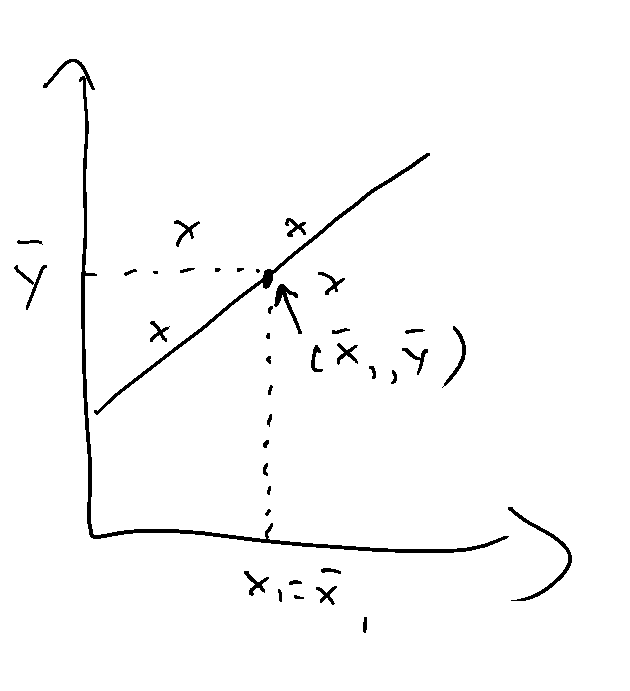
\includegraphics[width=.5\textwidth]{11.pdf}
\\ If $x_1 = \overline{x}_1$, we see that
$$m(\overline{x}_1) = \overline{y}$$
Thus the line \textbf{passes through} $\mathbf{(\overline{x}_1, \overline{y})}$. In comparison, the optimal line prediction (the
regression line) goes through $(E[X], E[Y])$.
\subsection{Bias, Variance and Standard Error of Parameter Estimators}
\paragraph{Estimator vs Estimates} An estimator is a random variable
and an estimate is a number (realized value of an estimator). E.g.\ we
can potentially draw $n$ samples.
$$X_1, X_2, \ldots, X_n$$
from a distribution, if $X_i$'s have not been actually observed yet,
then they can be viewed as random variables from that distribution.

Therefore the sample mean
\begin{align*}
  \overline{X} & = \dfrac{X_1 + \ldots + X_n}{n}
\end{align*}
is also a random variable, \textbf{called an estimator} of the
population mean $\mu$. But if the drawing has been conducted and the
values of $X_i$'s have been realized as $X_i = x_i, i = 1, \ldots, n$,
then the realized value
\begin{align*}
  \overline{x} & = \dfrac{X_1 + \ldots + X_n}{n}
\end{align*}
is an estimate of $\mu$.

Looking at the \href{https://yangyi.shinyapps.io/simulation/}{SLR
  simulation} on the course website, one can get a good idea as to how
the estimated $\beta$'s fluctuate with each different sample taken.
\\ \noindent \rule{\textwidth}{0.5pt}
We are going to prove the following statements:
\begin{align*}
  E[\hat{\beta}_1] & = \beta_1 & E[\hat{\beta}_0] & = \beta_0
  \\ Var(\hat{\beta}_1) & = \frac{\sigma^2}{S_{xx}} & Var(\hat{\beta}_0) & = \sigma^2 \left(\frac{1}{n} + \frac{\overline{x_1}^2}{S_{xx}}\right)
\end{align*}
First we find that the estimates
\begin{align*}
  \hat{\beta}_1 & = \frac{S_{xy}}{S_{xx}} = \dfrac{\sum_{i=1}^n (x_{1i} - \overline{x}_1)y_i}{S_{xx}} = \sum_{i=1}^n \underbrace{\dfrac{x_{1i} - \overline{x}_1}{S_{xx}}}_{= c_i}y_{i}
  = \sum_{i=1}^n c_i y_i
\end{align*}
With $c_i = \frac{(x_{1i} - \overline{x}_1)}{S_{xx}}, \sum_{i=1}^n c_i
= 0$. Similarly:
\begin{align*}
  \hat{\beta}_0 & = \overline{y} - \overline{x}_1 \hat{\beta}_1 = \overline{y} - \overline{x}_1 \sum_{i=1}^n c_i y_i
  \\ & = \frac{1}{n} \sum_{i=1}^n y_i - \overline{x}_1 \sum_{i=1}^nc_iy_i = \sum_{i=1}^{n} \underbrace{\left(\frac{1}{n} - \overline{x}_1 c_i\right)}_{b_i} y_i
\end{align*}
We find that both \textbf{estimates} are linear combinations of
$y_i$'s. The corresponding \textbf{estimators} of $\beta_0, \beta_1$
are formed by replacing the observed $y_i$ by the random variable
$Y_i$ in the previous formulas i.e.\
\begin{align*}
  \hat{\beta}_1 & = \sum_{i=1}^n c_i Y_i
  \\ \hat{\beta}_0 & = \sum_{i=1}^n \left(\frac{1}{n} - \overline{x}_1 c_i\right) Y_i
\end{align*}
In this section, we are going to treat $x_i$'s as \textbf{non-random}
variables. This is appropriate in designated or controlled
experiments, where we get to choose their values. But in randomized
experiments or in observational studies, obviously $x_i$'s are not
necessarily fixed. We will come back to how we get the
\textbf{unconditional expectation and variance} with $x_i$'s as random
variables.
\begin{align*}
  E[\hat{\beta}_1] & = E[\hat{\beta}_1 \mid x_{11}, \ldots, x_{1n}]
                     = E \left[\sum_{i=1}^n c_i Y_i \mid x_{11},\ldots, x_{1n}\right]
  \\ & = \sum_{i=1}^n c_i \underbrace{E \left[Y_i \mid x_{11}, \ldots,
       x_{1n}\right]}_{\text{if SLR assumptions true}}
  \\ & = \sum_{i=1}^n c_i E \left[\beta_0 + \beta_1 x_{1i} + \underbrace{\varepsilon_i}_{=0} \mid x_{11}, \ldots, x_{1n}\right]
  \\ & = \sum_{i=1}^n c_i (\beta_0 + \beta_1 x_{1i}) = \beta_0 \underbrace{\sum_{i = 1}^{n}c_i}_{= 0} + \beta_1 \underbrace{\sum_{i=1}^nc_i x_{1i}}_{=1} = \beta_1
\end{align*}
Since $\sum_{i=1}^n c_i = 0$ and
\begin{align*}
  \sum_{i=1}^n c_i x_{1i} & = \dfrac{\sum_{i=1}^n (x_{1i} - \overline{x}_1)x_{1i}}{S_{xx}} = \dfrac{\sum_{i=1}^n x_{1i}^2 - n (\overline{x}_1)^2}{S_{xx}} = 1
\end{align*}
Thus if we assume \textbf{the model is correct}; then $\beta_1$ is an
\textbf{unbiased} estimator of $\beta_1$. Similarly,
\begin{align*}
  E[\hat{\beta}_0] & = \beta_0
  \\ Var(\hat{\beta}_1) & = Var(\hat{\beta}_1 \mid x_{11}, \ldots, x_{1n}) = Var \left(\sum_{i=1}^n c_i Y_i \mid x_{11}, \ldots, x_{1n}\right)
  \\ & = \sum_{i=1}^n c_i^2 Var \left(Y_i \mid x_{11}, \ldots, x_{1n}\right)
\end{align*}
Because $Y_i$'s are uncorrelated and since
\begin{align*}
  Var \left(Y_i \mid x_{11}, \ldots, x_{1n}\right) & = Var (\beta_0 + \beta_1 x_{1i} + \varepsilon \mid x_{11}, \ldots, x_{1n})
  \\ & = \underbrace{Var (\beta_0 + \beta_1 x_{1i} \mid x_{11} , \ldots, x_{1n})}_{=0} + \underbrace{Var(\varepsilon \mid x_{11}, \ldots, x_{1n})}_{\sigma^2} = \sigma^2
\end{align*}
Consequently,
\begin{align*}
  Var(\hat{\beta}_1) & = \sigma^2 \sum_{i=1}^n c_i^2 = \sigma^2 \dfrac{\sum_{i=1}^n (x_{1i} - \overline{x}_1)^2}{S_{xx}^2} = \frac{\sigma^2}{S_{xx}}
\end{align*}
The variance of $\hat{\beta}_0$ is
\begin{align*}
  Var(\hat{\beta}_0) & = Var(\hat{\beta}_0 \mid x_{11}, \ldots, x_{1n}) = Var(\overline{Y} - \hat{\beta}_1 \overline{X}_1 \mid x_{11}, \ldots, x_{1n})
  \\ & = Var(\overline{Y} \mid x_{11}, \ldots, x_{1n}) + \underbrace{\overline{x}_1^2 Var(\hat{\beta}_1)}_{\frac{\sigma^2}{S_{xx}}} - 2 \overline{x}_1 Cov(\overline{Y}, \hat{\beta}_1 \mid x_{11}, \ldots, x_{1n})
  \\ & = \frac{\sigma^2}{n} + \overline{x}_1^2 Var(\hat{\beta}_1) + 0
       \intertext{
       Since $Var(Y_i) = \sigma^2, Var \left(\frac{Y_1 + \ldots + Y_n}{n}\right) =
       \frac{1}{n^2}\sigma^2 + \ldots + \frac{1}{n^2}\sigma^2 = \frac{\sigma^2}{n}$
       }
       & = \sigma^2 \left(\frac{1}{n} + \frac{\overline{x}_1}{S_{xx}}\right)
\end{align*}
\paragraph{Unconditional-on-$X$ properties} So far we have only computed
expectation and variance of $\hat{\beta}_1$ and $\hat{\beta}_0$
conditioned on $x_{11}, \ldots, x_{1n}$ either because the $x$'s are
not random or we're just interested in conditional inference. If we do
care about unconditional properties, we need to find
$E[\hat{\beta}_1]$ and $Var(\hat{\beta}_1)$, not just $E[\hat{\beta}_1
\mid x_{11}, \ldots, x_{n1}]$ and $Var(\hat{\beta}_1 \mid x_{11},
\ldots, x_{n1})$.

Use ``the law of total expectation''.
\begin{align*}
  E[\hat{\beta}_1] & = E_X [\underbrace{E_{Y \mid X} [\hat{\beta}_1 \mid X_{11}, \ldots, X_{1n}]}_{\beta_1}]
  \\ & = E_X [\beta_1] = \beta_1
\end{align*}
That is the estimator is \textbf{unconditionally unbiased}. To get the
unconditional variance, use ``the law of total variance''.
\begin{align*}
  Var(\hat{\beta}_1) & = E_X[Var(\hat{\beta}_1 \mid X_{11}, \ldots, X_{n1})] + Var_X[E_{Y \mid X} [\hat{\beta}_1 \mid X_{11}, \ldots, X_{1n}]]
  \\ & = E_X \left[\frac{\sigma^2}{S_{xx}}\right] + \underbrace{Var(\beta_1)}_{=0}
  \\ & = \sigma^2 E_X \left[\frac{1}{S_{xx}}\right]
\end{align*}
\subsection{Bias, variance of parameter estimators in matrix format}
Recall that if we denote
\begin{align*}
  Y & =
      \begin{bmatrix}
        Y_1 \\ \vdots \\ Y_n
      \end{bmatrix}, X =
  \begin{bmatrix}
    1 & X_{11}
    \\ \vdots & \vdots
    \\ 1 & X_{1n}
  \end{bmatrix}, \beta =
           \begin{bmatrix}
             \beta_0 \\ \beta_1
           \end{bmatrix}, \varepsilon =
  \begin{bmatrix}
    \varepsilon_1
    \\ \vdots
    \\ \varepsilon_n
  \end{bmatrix}
  \intertext{Thus we can rewrite the SLR model}
  Y_i & = \beta_0 + \beta_1 X_{1i} + \varepsilon_i, i = 1, \ldots, n
        \intertext{as}
        Y & = X\beta + \varepsilon
            \intertext{where}
            E[\varepsilon] & = 0 \text{ (vector)} \implies E[\varepsilon_i] = 0, i = 1, \ldots, n
  \\ Var(\varepsilon) & =
                        \begin{pmatrix}
                          Var(\varepsilon_1) & Cov(\varepsilon_1, \varepsilon_2)
                          \\ Cov(\varepsilon_2, \varepsilon_1) & \ddots
                          \\ & & Var(\varepsilon_n)
                        \end{pmatrix}
                                 = \sigma^2 I
                                 \intertext{Since $Var(\varepsilon_i)
                                 =\sigma^2$, $Cov(\varepsilon_j,
                                 \varepsilon_k) = 0, j \neq k$}
\end{align*}
We make the following observations:
\begin{itemize}
\item The true regression function is linear
  \begin{align*}
    E[Y \mid X] & = X \beta
                  \intertext{in the regular format, it is just}
                  E[Y_i \mid X_i = x_i] & = \beta_0 + \beta_1 x_i,\ i=1, \ldots, n
  \end{align*}
\item $Y$ has constant variance
  \begin{align*}
    Var(Y \mid X) & = \sigma^2 I,\ I = I_{n}
                    \intertext{Since}
                    Var(Y \mid X) & =
                                    \begin{bmatrix}
                                      Var(Y_1 \mid X) & Cov(Y_1, Y_2 \mid X) & \ldots & Cov(Y_1, Y_n \mid X)
                                      \\ Cov(Y_2, Y_1 \mid X) & Var(Y_2 \mid X) & & \vdots
                                      \\ \vdots & \ddots & \ddots
                                      \\ Cov(Y_n, Y_1 \mid X) & \ldots & \ldots & Var(Y_n \mid X)
                                    \end{bmatrix} = \sigma^2I
  \end{align*}
  This implies
  \begin{align*}
    Var(Y_i \mid X_i = x_i) & = \sigma^2,\ i=1, \ldots, n
    \\ Cov(Y_i, Y_j \mid X_i = x_i, X_j = x_j) & = 0,\ i \neq j
  \end{align*}
\end{itemize}
Now we can work on $\hat{\beta}$. We have that for the estimators
\begin{align*}
  \hat{\beta} & = \underbrace{(X^TX)^{-1}X^T}_{A}Y = A Y
                \intertext{Therefore}
                E[\hat{\beta} \mid X] & = E[AY \mid X]
                                        \intertext{Since $A$ consists
                                        only of terms of $X$, if we
                                        condition on $X$, then $A$ can
                                        be viewed as a constant}
  & = AE[Y \mid X] = (X^TX)^{-1}X^T E[Y \mid X]
  \\ & = \underbrace{(X^TX)^{-1}X^TX}_{I}\beta = \beta
\end{align*}
This is just $E[\hat{\beta}_0 \mid X] = \beta_0, E[\hat{\beta}_1 \mid
X] = \beta_1$.

For the variance:
\begin{align*}
  Var[\hat{\beta} \mid X] & = Var[AY \mid X]
                            \intertext{For scalars, we have $Var(\alpha
                            Y) = \alpha^2 Var(Y)$. For matrices, we have:}
  &= A \underbrace{Var[Y \mid X]}_{\sigma^2 I} A^T
    = A \sigma^2 I A^T
    = \sigma^2 A A^T
  \\ & = \sigma^2 ((X^TX)^{-1}X^T)((X^TX)^{-1}X^T)^{T}
       = \sigma^2 ((X^TX)^{-1}X^T)(X ((X^TX)^{-1})^{T})
  \\ & = \sigma^2 (X^TX)^{-1}X^TX ((X^TX)^{-1})^T
       = ((X^TX)^{-1})^T \stackrel{\text{$X^TX$ symmetric}}{=} (X^TX)^{-1}
  \\ &
       = \sigma^2 (X^TX)^{-1}
  \\ (X^TX)^{-1} & = \dfrac{1}{n \sum_{i=1}^nx_{1i}^2 - \left(\sum_{i=1}^nx_{1i}\right)^2}
                   \begin{bmatrix}
                     \sum_{i=1}^n x_{1i}^2 & - \sum_{i=1}^n x_{1i}
                     \\ -\sum_{i=1}^nx_{1i} & n
                   \end{bmatrix}
  \\ & = \dfrac{1}{n S_{xx}}
                   \begin{bmatrix}
                     \sum_{i=1}^n x_{1i}^2 & - \sum_{i=1}^n x_{1i}
                     \\ -\sum_{i=1}^nx_{1i} & n
                   \end{bmatrix}
  \\ Var(\hat{\beta} \mid X) & =
                               \begin{bmatrix}
                                 Var(\hat{\beta}_0 \mid X) & Cov(\hat{\beta}_0, \hat{\beta}_1 \mid X)
                                 \\ Cov(\hat{\beta}_1, \hat{\beta}_0 \mid X) & Var(\hat{\beta}_1 \mid X)
                               \end{bmatrix}
  \\ & = \sigma^2 (X^TX)^{-1}
       \intertext{This verifies}
  \\ Var(\hat{\beta}_0 \mid X) & = \dfrac{\sigma^2}{n} \dfrac{\sum_{i=1}^n x_{1i}^2}{S_{xx}} = \sigma^2 \left( \frac{1}{n} + \frac{\overline{x}_1^2}{S_{xx}}\right)
  \\ Var(\hat{\beta}_1 \mid X) & = \dfrac{\sigma^2}{S_{xx}}
  \\ Cov(\hat{\beta}_0, \hat{\beta}_1 \mid X) & = -\dfrac{\sigma^2 \sum_{i=1}^nx_{1i}}{n S_{xx}}
\end{align*}
\subsection{Residuals and additional properties}
The \textbf{residual} is defined as
\begin{align*}
  e_i & = y_i - \hat{y}_i,\ \hat{y}_i = \hat{\beta}_0 - \hat{\beta}_1 x_{1i}
\end{align*}
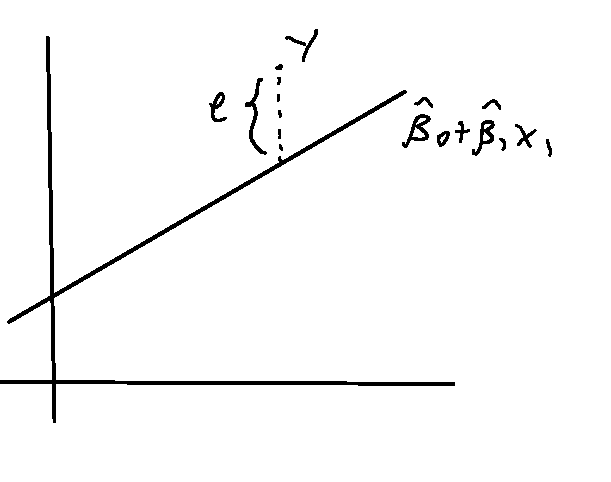
\includegraphics[width=.6\textwidth]{12.pdf}\\
Different from $\varepsilon$, this is the difference between the
regression line and point $y_i$, not the difference between the
regression line and the true regression line (that would be
$\varepsilon$).
\\ Recall that we have the normal equations:
\begin{align*}
  \frac{\partial{s}}{\partial{\beta_0}} & = \frac{1}{n}(-2) \sum_{i=1}^n (y_i - \underbrace{\hat{\beta}_0 - \hat{\beta}_1x_{1i}}_{\hat{y}_i}) = 0
  \\ \frac{\partial{s}}{\partial{\beta_1}} & = \frac{1}{n}(-2) \sum_{i=1}^n (y_i - \underbrace{\hat{\beta}_0 - \hat{\beta}_1x_{1i}}_{\hat{y}_i})x_{1i} = 0
\end{align*}
which is
\begin{align*}
  \sum_{i=1}^n(y_i - \hat{y}_i) & = \sum_{i=1}^ne_i =  0
  \\ \sum_{i=1}^n e_i x_{1i} & = 0
\end{align*}
Note:
\begin{itemize}
\item
  $\sum_{i=1}^n(y_i - \hat{y}_i) = \sum_{i=1}^ne_i =  0$
\item $\sum_{i=1}^n y_i = \sum_{i=1}^n \hat{y}_i$
\item $\sum_{i=1}^n x_{1i}e_i = 0$
\item $\sum_{i=1}^n \hat{y}_i e_i = 0$
\end{itemize}
The last equation is less obvious. To show it, we see that
\begin{align*}
  \sum_{i=1}^n \hat{y}_i e_i & = \sum_{i=1}^n (\hat{\beta}_0 + \hat{\beta}_1 x_{1i})e_{i} = \hat{\beta}_0 \underbrace{\sum_{i=1}^n e_i}_{=0} + \hat{\beta}_1 \underbrace{\sum_{i=1}^n x_{1i} e_i}_{=0}
  = 0
\end{align*}
\section{Estimating of $\sigma^2$}
Recall in the SLR:
\begin{align*}
  Y & = \beta_0 + \beta_1 X_1 + \varepsilon & E[\varepsilon] & = 0 & Var(\varepsilon) & = \sigma^2
\end{align*}
\begin{enumerate}
\item $\sigma^2$ captures the additional randomness in $y$.
\item $\sigma^2$ is in $Var(\hat{\beta}_0 \mid X)$ and
  $Var(\hat{\beta}_1 \mid X)$.
\end{enumerate}
\begin{align*}
  Var(\hat{\beta}_0 \mid X) & = \dfrac{\sigma^2}{n} \dfrac{\sum_{i=1}^n x_{1i}^2}{S_{xx}} = \sigma^2 \left( \frac{1}{n} + \frac{\overline{x}_1^2}{S_{xx}}\right)
  \\ Var(\hat{\beta}_1 \mid X) & = \dfrac{\sigma^2}{S_{xx}}
  \\ Cov(\hat{\beta}_0, \hat{\beta}_1 \mid X) & = -\dfrac{\sigma^2 \sum_{i=1}^nx_{1i}}{n S_{xx}}
\end{align*}
\paragraph{How to estimate $\sigma^2$?} Although $\sigma^2$ is not
used to compute $\hat{\beta}_0$ and $\hat{\beta}_1$, it is used to
understand the statistical properties of $\hat{\beta}_0$ and
$\hat{\beta}_1$.

We know that under SLR, it is easy to show that
\begin{align*}
  E[(Y - \beta_0 - \beta_1 X)^2] & = E[\varepsilon^2] = Var(\varepsilon) + (E[\varepsilon])^2
                                   = \sigma^2 + 0 = \sigma^2
\end{align*}
Idea: replace
\begin{itemize}
\item $Y$ with $y_i, i =1, \ldots, n$
\item $X_1$ with $x_{1i}, i = 1, \ldots, n$
\item $\beta_0$ with $\hat{\beta}_0$
\item $\beta_1$ with $\hat{\beta}_1$
\item $E$ with $\frac{1}{n} \sum_{i=1}^n$
\end{itemize}
To replace $E[(Y - \beta_0 - \beta_1 X_1)^2]$ with
$\frac{1}{n-2}\underbrace{\sum_{i=1}^n (y_i - \hat{\beta}_0 - \hat{beta}_1
x_{1i})^2}_{SS_{Res}}$.
\\ Let
\begin{align*}
  SS_{Res} & = \sum_{i=1}^n e_i^2 = \sum_{i=1}^n (y_i - \hat{y}_i)^2 = \underbrace{\sum_{i=1}^n (y_i - \hat{\beta}_0 - \hat{\beta}_1x_{1i})^2}_{S(\hat{\beta}_0, \hat{\beta}_1)}
\end{align*}
\begin{itemize}
\item ``Residual sum of squares''
\item Measures aggregate miss-fit of the least square line
\end{itemize}
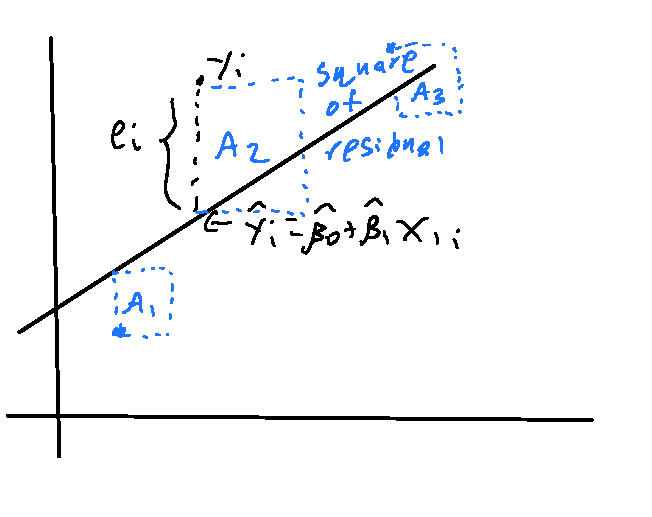
\includegraphics[width=.6\textwidth]{13.pdf}
\\ In this case, $SS_{Res} = A_1 + A_2 + A_3$. We see that the line
from least squares would minimize this.

The \textbf{unbiased estimator} for $\sigma^2$ is
\begin{align*}
  \hat{\sigma}^2 & = \dfrac{SS_{Res}}{n-2} = MS_{Res}
\end{align*}
$MS_{Res}$ is called the residual mean square.
\\ Note: $MSE$ vs $MS_{Res}$
\begin{align*}
  MSE & = \frac{1}{n} \sum_{i=1}^n (y_i - \beta_0 - \beta_1 x_{1i})^2
  \\ MS_{Res} & = \frac{1}{n-2} \sum_{i=1}^n (y_i - \hat{\beta}_0 - \hat{\beta}_1 x_{1i})
\end{align*}
We notice $n-2$ vs $n$ and also that we must use $\hat{\beta}_0,
\hat{\beta}_1$ from least squares, whereas for the $MSE$ it can be of
any form. If $n$ is very small, $MS_{Res}$ can have a large bias.

One can show that
\begin{align*}
  E[SS_{Res}] & = (n-2)\sigma^2
  \\ E[\hat{\sigma}^2] & = E \left[\frac{SS_{Res}}{n-2}\right] = \sigma^2
                   \text{ (unbiased)}
\end{align*}
\paragraph{Alternative formula for $SS_{Res}$}
\begin{align*}
  SS_{Res} & = \underbrace{\sum_{i=1}^n y_i^2 - n(\overline{y})^2}_{SS_T} - \hat{\beta}_1 S_{xy}
             \intertext{Let}
             SS_T & = \sum_{i=1}^n y_i^2 - n (\overline{y})^2 = \sum_{i=1}^n (y_i - \overline{y})^2
\end{align*}
$SS_T$ is called the ``\textbf{total sum of squares}''. Then
\begin{align*}
  SS_{Res} & = SS_T - \hat{\beta}_1 S_{xy}
\end{align*}
So we now know how to estimate $\hat{\beta}_0, \hat{\beta}_1,
\hat{\sigma}^2$. We now want to compute $E[\sigma^2]$ and
$Var(\sigma^2)$ like we already know for the other estimators. Note
that the proofs for these are very long and you do not need to
memorize the whole thing. Relevant parts (some intermediate steps will
provide lots of intuition and be useful for other things) will be highlighted in the notes on the
course website.
\subsection{Statistical properties of $\hat{\sigma}^2$ in matrix
  format}
Note: the quantity $SS_{Res}$ is an observed version of the
corresponding \textbf{random variable}
\begin{align*}
  \underbrace{\sum_{i=1}^n (y_i - \hat{y}_i)^2}_{SS_{Res}} & = (Y -
                                                             \hat{Y})^T
                                                             (Y -
                                                             \hat{Y})
                                                             = (Y - X
                                                             \hat{\beta})^T
                                                             (Y - X
                                                             \hat{\beta})
                                                             \text{ in
                                                             matrix format}
\end{align*}

We want to show that $\hat{\sigma}^2$ is an unbiased estimator.

Recall
\begin{align*}
  X\hat{\beta} & = \underbrace{X(X^TX)^{-1}X^T}_{H}Y = HY
\end{align*}
where $H$ is called the \textbf{hat matrix}
$$H = X(X^TX)^{-1}X^T \text{ ($n \times n$ matrix)}$$
\begin{itemize}
\item $H$ is a \textbf{symmetric} matrix
  $$H^T = X^T(X^TX)^{-1}X^T = H$$
\item $H$ is \textbf{idempotent}
  \begin{align*}
    H^T H & = HH = [X(X^TX)^{-1}X^T][X(X^TX)^{-1}X^T]
            = X(X^TX)^{-1}X^TX(X^TX)^{-1}X^T
    \\ & = X(X^TX)^{-1}X^T = H
  \end{align*}
\item $I_n - H$ is \textbf{idempotent}
  \begin{align*}
    I_n & =
          \begin{pmatrix}
            1 &&0
            \\ & \ddots
            \\ 0 & & 1
          \end{pmatrix}_{n \times n}
    \\ (I_n - H)^T (I_n-H) & = I_n^TI_n -I_n^T-H^T I_n + H^TH = I_n - H - H + H = I_n - H
                             \intertext{Therefore}
                             SS_{Res} & = (Y - X \hat{\beta}^T)(Y - X \hat{\beta})
                                        = (Y - HY)^T (Y - HY)
    \\ & = Y^T (I_n - H)^T(I_n - H)Y
         = Y^T (I_n - H)Y
  \end{align*}
\end{itemize}
  We need some tools to compute $E(SS_{Res})$. If $V$ is a random
  vector
  \begin{align*}
    E[V] & = \mu & Var(V) & = \Sigma
  \end{align*}
  Then we have that for a constant matrix $A$ (non-random):
  \begin{align*}
    E[V^TAV] & = trace(A \Sigma) + \mu^T A \mu
  \end{align*}
  Now we have $E[Y \mid X] = X \beta$ and $Var(Y \mid X) = \sigma^2
  I_n$.
  \begin{align*}
    E[SS_{Res} \mid X] & = E[\underbrace{Y^T}_{V^T} \underbrace{(I_n - H)}_A \underbrace{Y}_V \mid X] = trace((\underbrace{I_n - H}_A)\underbrace{\sigma^2 I_n}_{\Sigma}) + \underbrace{(X \beta)^T}_{\mu^T} \underbrace{(I_n - H)}_A \underbrace{(X \beta)}_\mu
    \\ & = \sigma^2 trace(I_n - H) + \beta^T X^T (I_n - H) X \beta
    \\ & = \sigma^2 trace (I_n - H) + \underbrace{\beta^T X^T (I_ - H)
         X\beta}_{= 0, \text{ see below}}
    \\ & = \sigma^2 trace (I_n) - \sigma^2 trace(H) + 0
         = \sigma^2 (n - trace(H))
         \intertext{Since}
         X^T(I_n - H)X & = X^T X - X^T H X
                         = X^T X - X^X(X^TX)^{-1} X^T X
    \\ & = X^TX - X^TX = 0
         \intertext{We know $trace (ABC) = trace(CAB) = trace(BCA)$
         (if dimension permits).}
         trace(H) & = trace(X(X^TX)^{-1}X^T) = trace(X^TX(X^TX)^{-1})
    \\ & = trace(I_p) = p
         \intertext{where $\mathbf{p = 2}$ \textbf{for simple linear
         regression}. The dimension of the matrix has changed from
         swapping terms, however because the matrix with
         multiplication swapped still exists, this is valid (dimension
         would not permit invalid multiplications, but it does allow
         changing the final dimension of the matrix)}
         E(SS_{Res} \mid X) & = E[Y^T (I_n - H)Y \mid X] = \sigma^2 (n-p) = \sigma^2 (n-2)
                              \intertext{Thus}
                              E[\hat{\sigma}^2 \mid X] & = E \left[\frac{SS_{Res}}{n-2} \mid X\right] = E \left[\frac{Y^T(I_n - H)Y}{n-2} \mid X\right]
    \\ & = \frac{\sigma^2 (n-2)}{n-2} = \sigma^2
  \end{align*}
  Note this is only true if our assumptions hold.

  \subsection{Use $\hat{\sigma^2}$ to estimate $Var(\hat{\beta}_0)$
    and $Var(\hat{\beta}_1)$}
  We can use $\hat{\sigma}^2$ to estimate $Var(\hat{\beta}_0 \mid X)$
  and $Var(\hat{\beta}_1 \mid X)$. Recall that the variance of
  $\hat{\beta}$ is
  \begin{align*}
    Var(\hat{\beta} \mid X) & =
                              \begin{pmatrix}
                                Var(\hat{\beta}_0 \mid X) & Cov(\hat{\beta}_0, \hat{\beta}_1 \mid X)
                                \\ Cov(\hat{\beta}_1, \hat{\beta}_0 \mid X) & Var(\hat{\beta}_1 \mid X)
                              \end{pmatrix} = \sigma^2 (X^TX)^{-1}
                                                                              \intertext{The
                                                                              diagonal
                                                                              entries
                                                                              can
                                                                              be
                                                                              written
                                                                              as}
                                                                              Var(\hat{\beta}_0 \mid X) & = \frac{\sigma^2}{n} \frac{\sum_{i=1}^n x_{1i}^2}{S_{xx}} = \sigma^2 \left(\frac{1}{n} + \frac{\overline{x}_1^2}{S_{xx}}\right)
    \\ Var(\hat{\beta}_1 \mid X) & = \frac{\sigma^2}{S_{xx}}
                                   \intertext{The standard errors (se)
                                   of the estimators are the square
                                   root of the variance.}
                                   SE(\hat{\beta}_0) & = \sqrt{Var(\hat{\beta}_0 \mid X)}
                                                       = \sqrt{\sigma^2 \left(\frac{1}{n} + \frac{\overline{x}_1^2}{S_{xx}}\right)}
    \\ SE(\hat{\beta}_1) & = \sqrt{Var(\hat{\beta}_1 \mid X)} = \sqrt{\frac{\sigma^2}{S_{xx}}}
                           \intertext{Replace $\sigma^2$ with known
                           $\hat{\sigma}^2$. Then we get
                           \textbf{estimated standard error (ese)}}
                           ese(\hat{\beta}_0) & = \sqrt{\hat{\sigma}^2 \left(\frac{1}{n} + \frac{\overline{x}_1}{S_{xx}}\right)}
    \\ ese(\hat{\beta}_1) & = \sqrt{\frac{\hat{\sigma}^2}{S_{xx}}}
  \end{align*}
  \section{Inference}
  Sampling distribution of $\hat{\beta}_0, \hat{\beta}_1$ and
    $\hat{\sigma}^2$.

    Recall that we derived
    \begin{align*}
      E[\hat{\beta}_1] & = \beta_1, & Var(\hat{\beta}_1) & = \frac{\sigma^2}{S_{xx}}, & E[\hat{\beta}_0] & = \beta_0, & Var(\hat{\beta}_0) & = \sigma^2 \left(\frac{1}{n} + \frac{\overline{x}_1^2}{S_{xx}}\right), & E[\hat{\sigma}^2] & = \sigma^2
    \end{align*}
    These results rely on the simple linear regression assumptions
    $E[\varepsilon \mid X_1 = x_1] =0$ and $Var(\varepsilon \mid X_1 =
    x_1) = \sigma^2$. But we still do not know the distribution of the
    estimator.

    But if we make some additional assumptions about the SLR models,
    i.e.\ Gaussian-Noise simple linear regression model in which we
    further assume an exact distribution for $\varepsilon$. This in
    turn can give us a conditional Gaussian distributed $Y$, which can
    then give us the sampling distribution of $\hat{\beta}_1,
    \hat{\beta}_0, \hat{\sigma}^2$. If $\varepsilon \sim N(0,
    \sigma^2)$, then
    \begin{align*}
      \hat{\beta}_1 & \sim N\left(\beta_1, \frac{\sigma^2}{S_{xx}}\right) & \hat{\beta_0} & \sim N \left(\beta_0, \sigma^2 \left(\frac{1}{n} + \frac{\overline{x}_1^2}{S_{xx}}\right)\right)
      \\ \frac{(n-2)\hat{\sigma}^2}{\sigma^2} & \sim \chi^2_{n-p}
                                                       \text{ ($p = 2$
                                                       for SLR)}
    \end{align*}
    \subsection{Gaussian-Noise simple linear regression model}
    (will be a question on exam)
    \\ Define \textbf{Gaussian-noise SLR} as
    \begin{enumerate}
    \item The distribution of $X$ is arbitrary (and perhaps $X$ is
      even non-random).
    \item $Y = \beta_0 + \beta_1 X_1 + \varepsilon$. If $X_1 = x_1$,
      then $Y = \beta_0 + \beta_1 x_1 + \varepsilon$, for some
      coefficients $\beta_0, \beta_1$ and some random noise
      $\varepsilon$.
    \item $\varepsilon \sim N(0, \sigma^2)$. Note that the original
      SLR assumptions were $E[\varepsilon] =0, Var(\varepsilon) =
      \sigma^2$. These still hold, however we have the additional
      assumption that it is Gaussian distributed.
    \item $\varepsilon$ is independent of $X_1$ and independent across observations.
    \end{enumerate}
    \begin{itemize}
    \item These assumptions are strictly stronger than the simple linear
      regression model. This means everything we have done so far
      directly applies to GN-SLR.
    \item First two assumptions are the same. The other assumptions
      have been made stricter:
      \\ $E[\varepsilon] = 0, Var(\varepsilon) = \sigma^2 \to
      \varepsilon \sim N(0, \sigma^2)$.
      \\ $\varepsilon$ is uncorrelated with $X_1 \to \varepsilon$ is
      independent to $X_1$ (independence implies uncorrelated, but not
      the other way around)
    \end{itemize}
    \subsection{Sampling distribution of $\frac{(\hat{\beta} -
        \beta)}{se(\hat{\beta})}$ and $\frac{(\hat{\beta} -
        \beta)}{ese(\hat{\beta})}$}
    Since
    \begin{align*}
      \hat{\beta}_1 & \sim N \left(\beta_1, \underbrace{\frac{\sigma^2}{S_{xx}}}_{Var(\hat{\beta}_1)}\right) & \hat{\beta}_0 & \sim N \left(\beta_0, \underbrace{\sigma^2 \left(\frac{1}{n} + \frac{\overline{x}_1^2}{S_{xx}}\right)}_{Var(\hat{\beta}_0)}\right)
    \end{align*}
    We are now going to standardize the random variables into standard
    normal distributions. We know
    that for a random variable $Z$, if $Z \sim N(\mu, \sigma^2)$ then
    \begin{align*}
      \frac{Z - \mu}{\sigma} & \sim N(0,1)
    \end{align*}
    Using the same idea,
    \begin{align*}
      \frac{\hat{\beta}_1 - \beta_1}{se(\hat{\beta}_1)} & \sim N(0,1) & \frac{\hat{\beta}_0 - \beta_0}{se(\hat{\beta}_0)} & \sim N(0,1)
      \\ se(\hat{\beta}_1) & = \sqrt{Var(\hat{\beta}_1)} = \sqrt{\frac{\sigma^2}{S_{xx}}} & se(\hat{\beta}_0) & = \sqrt{Var(\hat{\beta}_0)} = \sqrt{\sigma^2 \left(\frac{1}{n} + \frac{\overline{x}_1^2}{S_{xx}}\right)}
    \end{align*}
    The above two random variables follow $N(0,1)$, we could not
    directly use these to infer the unknown parameters $\beta_0,
    \beta_1$ since $se(\hat{\beta}_1), se(\hat{\beta}_0)$ are also
    unknown (because $\sigma^2$ is unknown). To solve this issue, we
    replace them with the \textbf{estimated standard error
      $\mathbf{ese(\hat{\beta}_1)}$ and $\mathbf{ese(\hat{\beta}_0)}$}

    We can show that $T_1 = \frac{\hat{\beta}_1 -
      \beta_1}{ese(\hat{\beta}_1)} \sim t_{n-p}, T_0 =
    \frac{\hat{\beta}_0 - \beta}{ese(\hat{\beta}_0)} \sim t_{n-p}$,
    where $p = 2$ for GN-SLR.
    \\ \noindent \rule{\textwidth}{0.5pt}
    You will not have to write R code for the midterm, however, you
    might have to interpret code output (look at
    \href{http://www.math.mcgill.ca/yyang/regression/comp/Comp-05-estimation_sigma.pdf}{\texttt{Comp-05-estimation\_sigma.pdf}}
    and interpret the results of \texttt{lm} and more), like what the sample mean
    means and whatnot. Focus on assignment and notes, midterm covers
    everything up to midterm's class.
    \\ \noindent \rule{\textwidth}{0.5pt}
    Notice that we can compute $ese(\hat{\beta}_1) =
    \sqrt{\frac{MS_{Res}}{S_{xx}}}$ and $ese(\hat{\beta}_0) =
    \sqrt{MS_{Res} \left(\frac{1}{n} +
        \frac{\overline{x}_1^2}{S_{xx}}\right)}$ from the data without
    knowing the true parameter $\sigma^2$.
    \section{Confidence Intervals}
    First we construct the CI for $\beta_1$. Suppose that $f_T$ is the
    density of a $T \sim t_{n-2}$ distribution, defined
    $$k \equiv t_{\frac{\alpha}{2}, n-2} > 0$$
    such that
    \begin{align*}
      P(-k \leq T \leq k) & = \underbrace{1 - \alpha}_{=0.95 \text{ if
                            } \alpha = 0.05}, \alpha \in (0,1), \alpha
                            \text{ is user specified}
    \end{align*}
    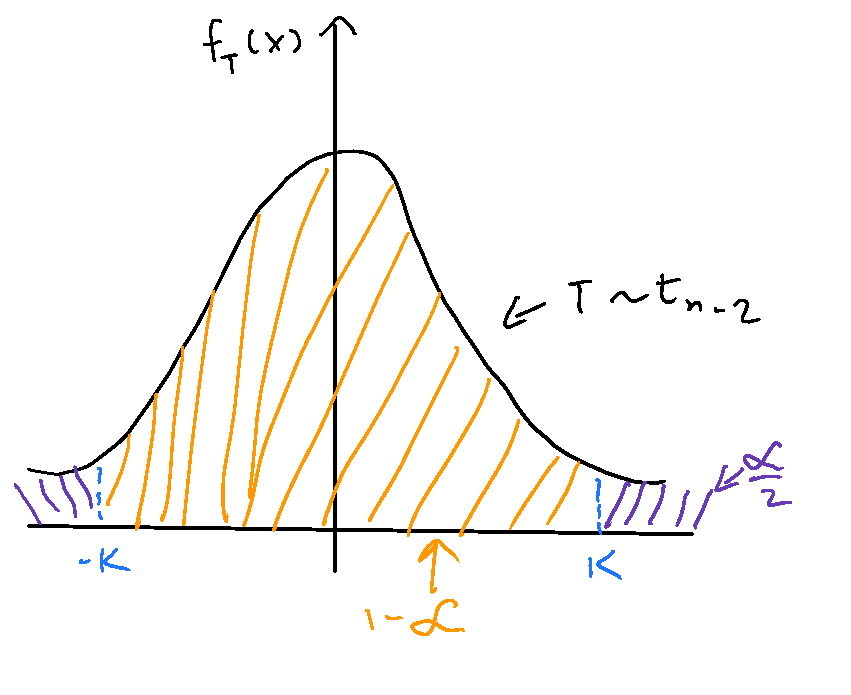
\includegraphics[width=.6\textwidth]{14.pdf}
    \\ A $100(1 - \alpha)\%$ level confidence interval \underline{for
      $\beta_1$} (not $\hat{\beta}_1$) is defined as
    \begin{align*}
      CI(\beta_1) & = [\hat{\beta}_1 - k \cdot ese(\hat{\beta}_1), \hat{\beta}_1 + k \cdot ese(\hat{\beta}_1)]
                    \intertext{To verify this, note that}
                    P(\beta_1 \in CI(\beta_1)) & = P(\hat{\beta}_1 - k \cdot ese(\hat{\beta}_1) \leq \beta_1 \leq \hat{\beta}_1 + k \cdot ese(\hat{\beta}_1))
      \\ & = P \left(-k \leq \underbrace{\frac{\hat{\beta}_1 - \beta_1}{ese(\beta_1)}}_{T_1} \leq k\right)
           = 1 - \alpha
    \end{align*}
    Note:
    \begin{itemize}
    \item The upper and lower bound of $CI(\beta_1)$ are
      \textbf{random}, since their formula involves the estimator
      $\hat{\beta}_1$ which could potentially be random if
      $\hat{\beta}_1$ is computed using a different set of samples
    \item Interpretation: The interval $CI(\beta_1)$ traps $\beta_1$
      with probability $1 - \alpha$ (this will be on the midterm).
    \item $\beta_1$ is \textbf{non-random}
    \item Notice that the width of the confidence interval is $2 \cdot
      k \cdot ese(\hat{\beta}_1)$.
      \begin{itemize}
      \item
        As $\alpha$ shrinks, the interval
        widens (to be more certain about including $\beta_1$, you must
        make the interval larger).
      \item As $n$ grows, the interval shrinks.
      \item As $\sigma^2$ increases, the interval widens.
      \item As $S_{xx}$ grows, the interval shrinks.
        \begin{align*}
          ese(\hat{\beta}_1) & = \sqrt{\frac{MS_{Res}}{S_{xx}}} & S_{xx} & = \sum_{i=1}^n (x_i - \overline{x})^2
        \end{align*}
        If the data is well spread, the interval shrinks (you have
        more points from everywhere). Intuitively, when the points are
        more clustered together, changing the data of one point/adding
        one point will greatly modify the regression line, but if
        they're further apart it won't change as much.\\
        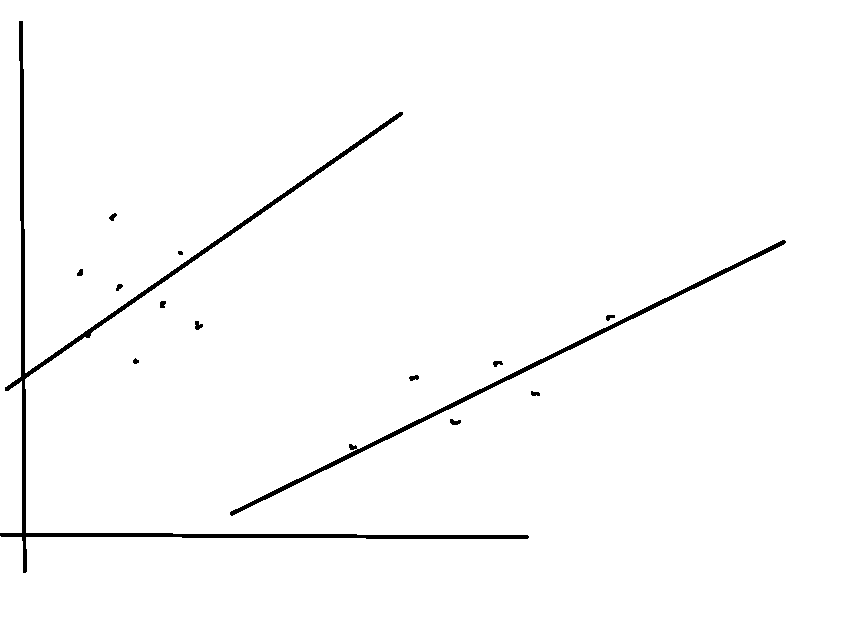
\includegraphics[width=.6\textwidth]{15.pdf}
      \end{itemize}
    \end{itemize}
    What about $CI(\beta_0)$? By parallel reasoning, a $1- \alpha\
    CI(\beta_0)$ is
    \begin{align*}
      CI(\beta_0) & = [\hat{\beta}_0 - k \cdot ese(\hat{\beta}_0), \hat{\beta}_0 + k \cdot ese(\hat{\beta}_0)]
    \end{align*}
    If you have already calculated $k$ from $CI(\beta_1)$, you won't
    need to recalculate it here.
    \subsection{Hypothesis Testing}
    Suppose we want to test (two sided test)
    \begin{align*}
      H_0: & \beta_1 = c
      \\ H_1: & \beta_1 \neq c
    \end{align*}
    where $c$ is a specific value, e.g.\ $c$ can be $0$.

    Rule: we reject $H_0$ in a hypothesis test with significance level
    $\alpha$, if the $100(1- \alpha)\%$ confidence interval
    $CI(\beta_1)$ \textbf{does not} cover $c$.

    Why: As an example, let's set $\alpha = 0.01$. If $H_0$ is true,
    then its highly likely (with probability $1 - \alpha = 0.99$)
    $CI(\beta_1)$ should trap $\beta_1 = c$. So if we observe that
    $CI(\beta_1)$ does not trap $c$, it could be either
    \begin{itemize}
    \item $\beta_1 = c$ ($H_0$ is true) and therefore we just (by
      chance) observed a very rare event that $CI(\beta_1)$ does not
      trap $\beta_1 = c$ (with probability $\alpha$), this is a type
      $1$ error (false rejection)
    \item or $\beta_1 \neq c$ and $H_0$ should be rejected
    \end{itemize}
    If we reject $H_0$ when $CI(\beta_1)$ does not cover $c$, it is
    equivalent to
    \begin{align*}
      c \notin CI(\beta_1) & \iff c \geq \hat{\beta}_1 + k \cdot
                          ese(\hat{\beta}_1) < k \text{ or } c \leq \hat{\beta}_1 - k \cdot ese (\hat{\beta}_1)
      \\ & \iff \frac{\hat{\beta}_1 - c}{ese(\hat{\beta}_1)} \text{ or
           } \frac{\hat{\beta}_1 - c }{ese(\hat{\beta}_1)} \geq k
      \\ & \iff |T_1| \geq k \equiv t_{\frac{\alpha}{2}, n-2}, \underbrace{T_1 = \frac{\hat{\beta}_1 - c }{ese(\hat{\beta}_1)}}_{\text{t-statistic}} \stepcounter{equation}\tag{*}\label{eq:1}
    \end{align*}
    This is called Wald test or t-test and $T_1$ is called \textbf{t
      test statistics}.
    \\
    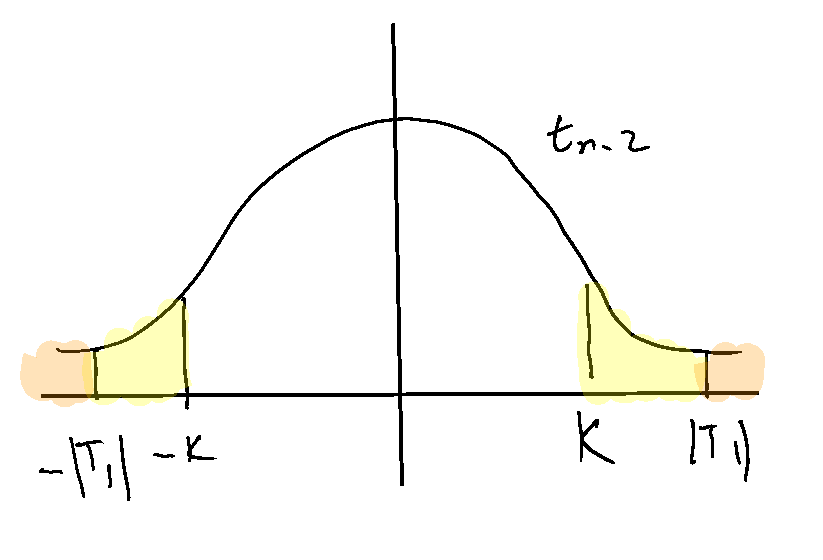
\includegraphics[width=.6\textwidth]{16.pdf}
    \begin{align*}
      (\ref{eq:1}) & \iff \text{Orange Area} \leq \text{Yellow Area}
      \\ & \iff \underbrace{Pr(|T| > |T_1|)}_{\text{Orange Area,
           $p$-value}} < \underbrace{\alpha}_{\text{Yellow Area}}
    \end{align*}

    What about a test for $\beta_0$?
    \begin{align*}
      H_0: & \beta_0 = c
      \\ H_1: & \beta_0 \neq c
    \end{align*}
    By the same reasoning, we reject $H_0$ if
    \begin{align*}
      |T_0| & \geq k \equiv t_{\frac{\alpha}{2}, n-2} & T_0 & = \frac{\hat{\beta}_0- c}{ese(\hat{\beta}_0)}
    \end{align*}
    \subsubsection{Testing significance of regression}
    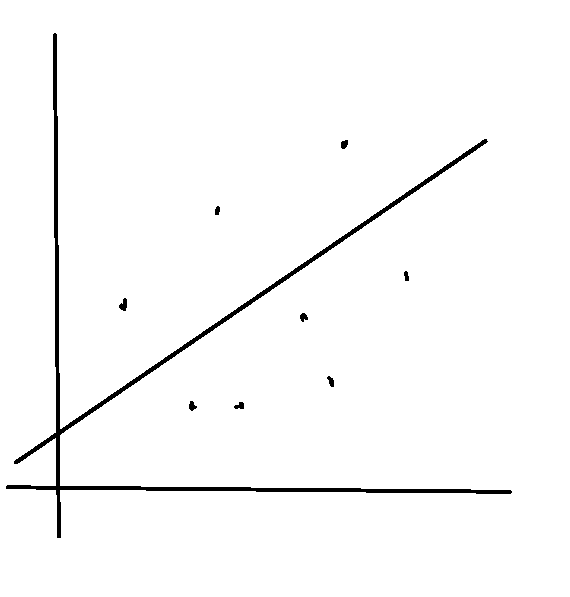
\includegraphics[width=.6\textwidth]{17.pdf}
    \begin{align*}
      H_0: & \beta_1 = 0
      \\ H_1: & \beta_1 \neq 0
    \end{align*}
    This hypothesis test is related to the significance of regression.

    Failing to reject $H_0: \beta_1 = 0$ implies that there is
    \textbf{no linear relationship} between $X_1$ and $Y$.
    \begin{itemize}
    \item Either $X_1$ is of little value in explaining the variation
      in $Y$
    \item Or the true relationship between $X_1$ and $Y$ is not linear
    \end{itemize}
    We reject $H_0$ with significance level $\alpha$ if the
    $100(1-\alpha)$ percent confidence interval $CI(\beta_1)$ does
    not cover $0$.

    The corresponding test statistic is:
    \begin{align*}
      T_1 & = \frac{\hat{\beta}_1 - c}{ese(\hat{\beta}_1)} =
            \frac{\hat{\beta}_1}{ese(\hat{\beta}_1)}\ (c = 0, \text{
            special case})
    \end{align*}
    We reject $H_0:\beta_1 = 0$ if $|T_1| > k \equiv
    t_{\frac{\alpha}{2}, n - 2}$
    \\ \noindent \rule{\textwidth}{0.5pt}
    \paragraph{Some review of midterm questions}
    ~\\
    \begin{tabular}{l | l | l}
      & SLR & GN-SLR
      \\\hline Estimation $\hat{\beta}_1, ese(\hat{\beta}_1), \hat{\sigma}^2$ & \checkmark & \checkmark (not necessary)
      \\ Unbiasness. $E(\hat{\beta}_1)$ and Var $Var(\hat{\beta}_1)$ & \checkmark & \checkmark (not necessary)
      \\ Confidence Intervals & & \checkmark
      \\ Hypothesis testing $t$-test & & \checkmark
      \\ F-test & & \checkmark
      \\ Prediction interval & & \checkmark
    \end{tabular}
    \\ \noindent \rule{\textwidth}{0.5pt}
    \subsection{Statistical Significance}
    \begin{itemize}
    \item What $\alpha$ should we use? Conventionally, set $\alpha =
      0.05$. If you are very conservative and can't afford false
      rejection, you should use a smaller $\alpha$.
    \item Statistical significance: if we test the hypothesis that
      \begin{align*}
        H_0: \beta_1 = 0
      \end{align*}
      and reject it, we say the difference between $\beta_1$ and $0$ is
      \textbf{statistically significant}.
    \item Statistical significance $\neq$ importance of magnitude

      When $H_0$ is attained, it should be interpreted as
      ``\textbf{the effect of $\mathbf{\beta_1}$ is statistically
        undetectable}'' or ``\textbf{$\mathbf{\beta_1}$ is
        statistically undistinguishable from $\mathbf{0}$}''
      $$\left|\frac{\hat{\beta}_1}{ese(\hat{\beta}_1)}\right| > k$$
      The effect might be huge or small, can't detect it. Failing to
      reject is very conservative, can't say much. However if you fail
      to reject, it is a very strong claim.
    \item e.g.\ a common fallacy is ``I tested whether $H_0 = \beta_1
      = 0$ or not, and I retain $H_0$, therefore $\beta_1$ is
      insignificant, and it is unimportant and you can ignore
      it''. Because we retain $H_0: \beta_1 = 0$ when $\left|
        \frac{\hat{\beta}_1}{ese(\hat{\beta}_1)}\right| < k$, there
      are two cases that might result in a rejection of $H_0$.
      \begin{enumerate}[(1)]
      \item $\hat{\beta}_1$ is very close to zero, which implies
        $\beta_1$ may as well be zero, thus unimportant.
      \item $ese(\hat{\beta}_1)$ is so large that we can't tell
        anything about $\beta_1$ with any confidence ($\beta_1$ may be
        either large or small).
      \end{enumerate}
      This is a \underline{false/bad} claim (fallacy) because you don't have
      enough evidence to say it is unimportant or make any claim. It
      might potentially be important.
    \end{itemize}
    \section{Analysis of Variance (ANOVA)}
    We can use the ``\textbf{analysis of variance}'' approach to test
    the significance of regression.

    The distance from any point $y_i$ in a collection of data to
    $\overline{y}$ is the deviation, written as $y_i - \overline{y}$.
    The ANOVA is based on a partition of total variability in $y$.
    $$y_i - \overline{y} = (y_i - \hat{y}_i) + (\hat{y}_i -
    \overline{y})$$
    where $\hat{y}_i = \hat{\beta}_0 + \hat{\beta}_1 x_{1i}$. One can
    show that
    \begin{align*}
      \underbrace{\sum_{i=1}^n (y_i - \overline{y})^2}_{SS_T} & = \underbrace{\sum_{i=1}^n (y_i - \hat{y}_i)^2}_{SS_{Res}} + \underbrace{\sum_{i=1}^n (\hat{y}_i - \overline{y})^2}_{SS_R}
    \end{align*}
    \begin{itemize}
    \item $SS_T$ --- total sum of squares. It measures ``total
      variation'' in $Y$.
    \item $SS_{Res}$ --- Residual sum of squares. It measures the
      amount of ``residual variation'' in $Y$. It is an aggregate
      measure of mis-fit of the fitted regression line.
    \item $SS_R$ --- regression sum of squares. It measures amount of
      ``systematic variation'' in $Y$ due to the $y \sim x$ linear relationship.
    \end{itemize}
    \begin{minipage}{.5\linewidth}
    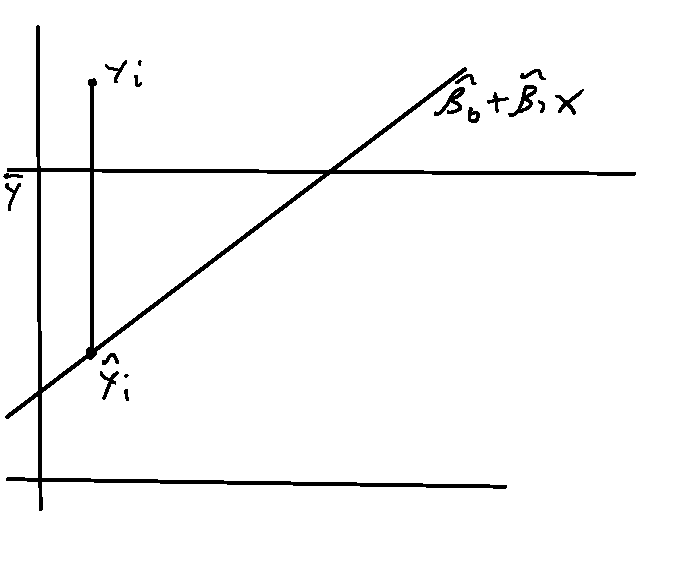
\includegraphics[width=\textwidth]{18.pdf}
    \end{minipage}
    \begin{minipage}{.5\linewidth}
    \begin{align*}
      y_1 \ldots y_n& & \overline{y} & = \frac{\sum_{i=1}^n y_i}{n}
      \\ y_i - \overline{y} & = (y_i - \hat{y}_i) + (\hat{y}_i - \overline{y})
    \end{align*}
  \end{minipage}
  \begin{itemize}
  \item $SS_T = \sum_{i=1}^n (y_i - \overline{y})^2$
    \\ 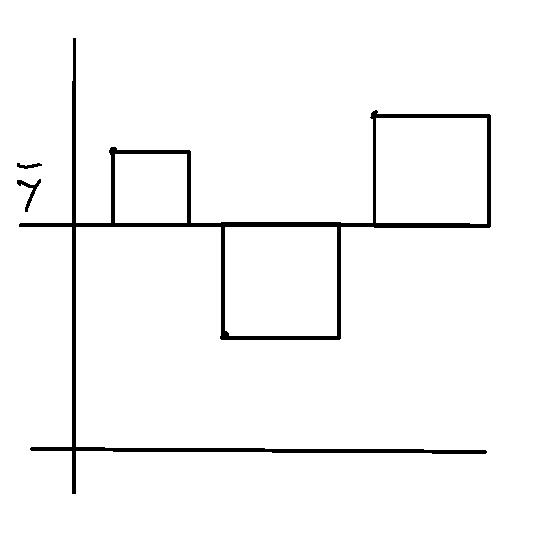
\includegraphics[width=.5\textwidth]{19.pdf}
  \item $SS_{Res} = \sum_{i=1}^n (y_i - \hat{y}_i)^2$
    \\ 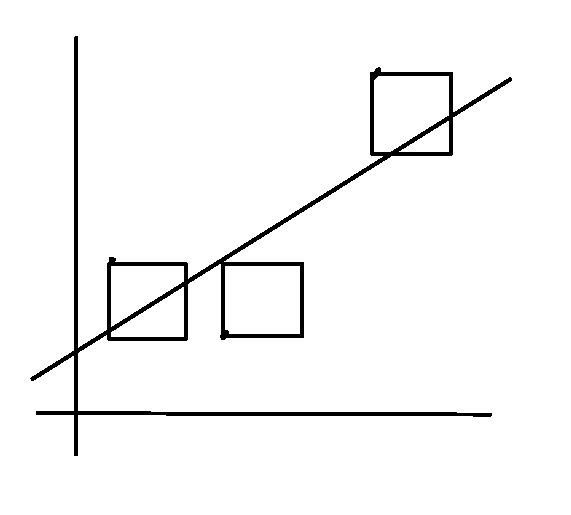
\includegraphics[width=.5\textwidth]{20.pdf}
  \item $SS_R = \sum_{i=1}^n (\hat{y}_i - \overline{y})^2$
    \\ 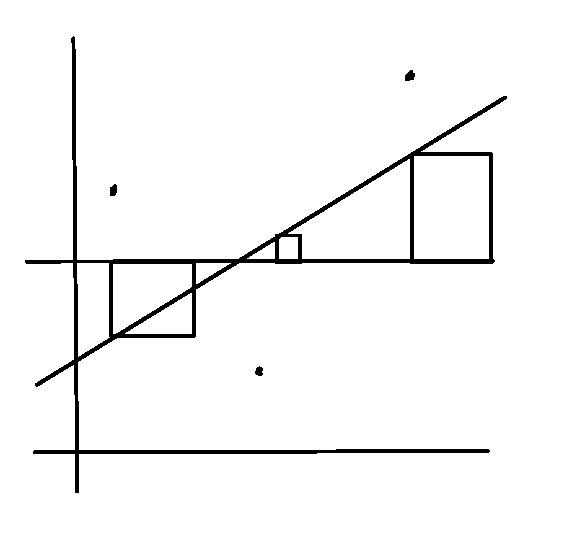
\includegraphics[width=.5\textwidth]{21.pdf}
  \end{itemize}
  \paragraph{Proof}
  \begin{align*}
    \underbrace{\sum_{i=1}^n (y_i - \overline{y})^2}_{SS_T} & = \sum_{i=1}^n (y_i - \hat{y}_i + \hat{y}_i - \overline{y})^2
    = \sum_{i=1}^n (\underbrace{(y_i - \hat{y}_i)}_{e_i} + (\hat{y}_i - \overline{y}))^2 \\
                                        & = \sum_{i=1}^n ((\hat{y}_i - \overline{y})^2 + 2e_i (\hat{y}_i - \overline{y}) + e_i^2)
                                          = \underbrace{\sum_{i=1}^n (\hat{y}_i - \overline{y})^2}_{SS_R} + \underbrace{\sum_{i=1}^n e_i^2}_{SS_{Res}} + \underbrace{2 \sum_{i=1}^n e_i (\hat{y}_i - \overline{y})}_{=0} \\
                                                            & = \sum_{i=1}^n (\hat{y}_i - \overline{y})^2 + \sum_{i=1}^n e_i^2 + 2 \sum_{i=1}^n e_i (\hat{\beta}_0 + \hat{\beta}_1x_{1i} - \overline{y})
 \\
                                                              & = SS_R + SS_{Res} + 2(\hat{\beta}_0 - \overline{y}) \underbrace{\sum_{i=1}^n e_i}_{=0} + 2 \hat{\beta}_1 \underbrace{\sum_{i=1}^n e_i x_{1i}}_{=0}
  \end{align*}
  \section{F-test}
  The idea is to compare two models
  $$H_0: Y = \beta_0 + \varepsilon \text{ versus } H_1: Y = \beta_0 +
  \beta_1 X_1 + \varepsilon$$
  or equivalently,
  $$H_0: \beta_1 = 0 \text{ versus } H_1: \beta_1 \neq 0$$
  If we fit the first model, the least
\end{document}